\documentclass[a4paper,11pt]{article}
\pdfoutput=1 % if your are submitting a pdflatex (i.e. if you have
             % images in pdf, png or jpg format)

\usepackage{jinstpub} % for details on the use of the package, please
                     % see the JINST-author-manual

\usepackage[colorinlistoftodos]{todonotes}

\usepackage{epsfig}
\usepackage{amssymb}
\usepackage{subfigure}
\usepackage{lineno}
\usepackage{amsmath}
\usepackage{siunitx}
\usepackage[colorlinks=true,
            linkcolor=red,
            urlcolor=blue,
            citecolor=green]{hyperref}
\usepackage{url}
\usepackage{textgreek}
\usepackage{booktabs}

% The number `e'
\providecommand*{\eu}%
{\ensuremath{\mathrm{e}}}

% The imaginary unit
\providecommand*{\iu}%
{\ensuremath{\mathrm{j}}}

%define differential
\makeatletter
\providecommand*{\diff}%
{\@ifnextchar^{\DIfF}{\DIfF^{}}}
\def\DIfF^#1{%
\mathop{\mathrm{\mathstrut d}}%
\nolimits^{#1}\gobblespace}
\def\gobblespace{%
\futurelet\diffarg\opspace}
\def\opspace{%
\let\DiffSpace\!%
\ifx\diffarg(%
\let\DiffSpace\relax
\else
\ifx\diffarg[%
\let\DiffSpace\relax
\else
\ifx\diffarg\{%
\let\DiffSpace\relax
\fi\fi\fi\DiffSpace}

\linenumbers

\usepackage{titlesec}
\titleformat{\paragraph}[runin]
{\bfseries\scshape}{\theparagraph}{1em}{}
\setcitestyle{square}

\date{\today}

\title{Journal of Instrumentation (JINST) template}


%% %simple case: 2 authors, same institution
%% \author{A. Uthor}
%% \author{and A. Nother Author}
%% \affiliation{Institution,\\Address, Country}

% more complex case: 4 authors, 3 institutions, 2 footnotes
\author[a,b,1]{Laura Manenti,\note{Corresponding author.}}
\author[b]{Anastasia Basharina-Freshville,}
\author[b]{Francesco Arneodo,}
\author[b]{Mario Campanelli,}
\author[b]{Linda Cremonesi,}
\author[b]{Sameer Al-Kilani,}
\author[b]{Ryan Nichol,}
\author[b]{Ruben Saakyan}

% The "\note" macro will give a warning: "Ignoring empty anchor..."
% you can safely ignore it.

\affiliation[a]{One University,\\some-street, Country}
\affiliation[b]{Another University,\\different-address, Country}

% e-mail addresses: only for the corresponding author
\emailAdd{laura.manenti@ucl.ac.uk}




\abstract{Abstract...}



\keywords{Only keywords from JINST's keywords list please}


\arxivnumber{1234.56789} % only if you have one


% \collaboration{\includegraphics[height=17mm]{example-image}\\[6pt]
%   XXX collaboration}
% or
%\collaboration[c]{on behalf of XXX collaboration}


% if you write for a special issue this may be useful
%\proceeding{N$^{\text{th}}$ Workshop on X\\
%  when\\
%  where}



\begin{document}
\maketitle
\flushbottom

%**********************************************
\section{Introduction}
%**********************************************
%Here we give an intro to the PM: in which context it will be used and what it is. Briefly talk about previous works and what's new in our work. 

Liquid Argon Time Projection Chambers (LAr-TPCs) are the detection technology foreseen for the Far Detectors (FD) in the Deep Underground Neutrino Experiment (DUNE). 
%DUNE aims at studying long-baseline neutrino oscillations arising from neutrinos produced at the Fermi National Accelerator Laboratory and detected \SI{1300}{\km} away by \SI{40000}{\tonne} of liquid argon split among four detectors at the Sanford Underground Research Laboratory.
An R\&D programme currently underway at CERN operates two prototype detectors of the kind that will be employed by DUNE. Both use LAr-TPCs as detection technique, with one prototype, called Single-Phase (SP) protoDUNE, only using liquid argon, and the other, named Dual-Phase (DP) protoDUNE, using argon in both its gaseous and liquid state.
%The aim of the CERN R\&D programme is to test the prototypes design, assembly and installation procedures, the detectors operations, as well as data acquisition, storage, processing and analysis.
The work presented in this paper is part of the dual-phase protoDUNE effort. In a dual-phase LAr-TPC the ionisation charge is drifted upwards and extracted into the gaseous phase. Here, Large Electron Multipliers (LEMs) amplify the charge signal which is then read by the anode, allowing for a 2D image reconstruction of the track. It is obvious that high purity is needed for the ionisation charge to reach the LAr surface in the first place. 
With a drift distance of \SI{\approx 6}{\m}, the DP protoDUNE needs an electron lifetime of at least \SI{6}{ms}, which requires electronegative impurities in the liquid to be below the ppb level. 

Although the detector itself can estimate the purity of the liquid by measuring the charge deposited by muon tracks, this depends on the availability of muons traversing the TPC (whose frequency is greatly reduced underground) and is only possible when the cryostat is fully filled and a certain level of purity is achieved. Moreover, space-charge effects may distort the lifetime measurement. In fact, for each electron drifting to the cathode, there is a positive ion drifting to the anode. But, as positive ions are about one hundred-thousand times slower than electrons and the flow of cosmic muons is continuous, positive charges accumulate in the TPC. This charge build-up, usually referred to as space-charge, leads to field lines distortions and, subsequently, to distortions in the reconstructed track image. The effect is greater for bigger TPC volumes and at lower fields.
Commercially available Residual Gas Analysers (RGAs) are generally used for analysing the gas argon purity in the cryostat ullage, but are unsuitable to measure the purity of the liquid, as their sensitivity only goes down to the \SI{\approx 10}{ppb}. 
That is why custom-made devices, called purity monitors, have been designed and constructed. These will be installed at the bottom of cryostat and will continuously measure the LAr purity during the DP protoDUNE commissioning and operation phases. 
%Besides the fact that it is good to know the purity of the liquid, is there any other reason you need PMs? For correcting the energy deposition, but I guess for that you use muons...
Purity monitoring is especially useful while filling the cryostat and when recirculation is turned on: at that point electronegative impurities should constantly drop over time until stable operation conditions are reached. 
Because of the scale of the detector, sudden changes in the purity might go unnoticed, putting to risk the detector data taking. Purity monitors also mitigate against such risks. 

Purity monitors have so far been successfully deployed in the ICARUS, MicroBooNE, 35t~\cite{IDRvol2}, and SP protoDUNE detectors.
The purity monitor presented in this work closely resembles the ICARUS design with a few---fundamental---modifications.

%Explain in two lines how they work. That you need light to emit the electrons, but light suffers from attenuation. This means that better cathodes are the KEY. That's why this work. 
A purity monitor works by generating electrons from a cathode and drifting them towards an anode. The attenuation in the charge from cathode to anode gives a direct measurement of the electron lifetime in the liquid. 
It is common practice to produce the electrons at the cathode in the following way: a xenon flash lamp is placed outside the cryostat and coupled through a quartz optical fibre to a gold-coated cathode, where the UV photons extract electrons by photoelectric effect.
One major caveat of this setup is that only a tiny portion of the photons emitted by the xenon flash lamp---which has a broad spectrum range between 200 and \SI{2000}{nm}---can extract photons from the gold, namely the ones whose energy exceeds the gold work function, i.e. $\approx$\SI{5.1}{\eV} or equivalently $\approx$\SI{243}{nm}. Moreover, as the intensity of the flashes is attenuated by \SI{1}{\dB} for every \SI{1}{m} of optical fibre, less and less photons make it to the cathode from the lamp. 

This work compares for the first time the performance of various photocathodes, specifically gold, titanium, silver, and aluminium. Our results show that silver gives the best results in liquid argon, with the silver signal being x bigger than gold (which has always been the ``standard'' choice for LAr purity monitors). This is very useful especially in light of DUNE, where purity monitors at the bottom of the cryostat may only work if enough electrons are emitted by the photocathode in the first place. 
The possibility of using the purity monitor with a \SI{25}{m} quartz fibre is also established for the first time.  

%**********************************************
\section{Experimental setup}
%**********************************************
\subsection{The purity monitor}
The xenon flash lamp is the L7685 from Hamamatsu. The lamp comes with a cooling jacket (p/n~E6611) which hosts the xenon bulb, a trigger socket (p/n E6647) and power supply (p/n C6096-02) which provide the high voltage to trigger the spark of the gas in the bulb, and an external discharge capacitor (p/n E7289-02) which allows the lamp to run at \SI{1}{\joule} per flash. A \SI{24}{V_{dc}} voltage with a capacity of \SI{3}{A} is supplied externally to both the cooling jacket and the power supply. The lamp may be triggered in external or internal mode. For the latter, an internal trimmer may be adjusted to set the flash repetition rate. In this work, the lamp was triggered externally by using a pulse generator (pulse mode, at \SI{5}{Hz}, with \SI{5}{V_{PP}} in amplitude, and \SI{1}{\micro s} in width) connected to the Hamamatsu trigger socket. The pulse generator also provided the trigger to the oscilloscope. 

The optical fibre which couples the cathode to the lamp is made of fused silica and coated in Polyimide. It has a core diameter of \SI{600}{\micro m} and is transparent in the 190--\SI{1250}{nm} range. The minimum (continuous) bending radius is \SI{132}{mm} which makes the fibre quite fragile to handle. According to the supplier's datasheet, the attenuation at \SI{\approx 250}{nm} is \SI{\approx 0.3}{dB\per\metre}, meaning that for a \SI{25}{m} long fibre the light loss due to attenuation is of around 80\%. 
%http://www.timbercon.com/db-power-loss/

%%%% TABLE CATHODES %%%%
\begin{table}[tb]
\centering
\caption[]{The table summarises the properties of the photocathode coatings tested. Note that the gold photocathode needs a $\approx$\SI{5}{nm} Ti substrate for the gold to adhere. All the depositions have been performed at the London Centre for Nanotechnology.}
    
    \smallskip
    \begin{tabular} {@{}lrlccc@{}}
    \toprule
    \multicolumn{1}{c}{Technique} &\multicolumn{2}{c}{Material} &\multicolumn{1}{c}{Pressure[mbar]} &\multicolumn{1}{c}{Dep. rate [nm/s]} &\multicolumn{1}{c}{Thickness [nm]} \\
    \cmidrule(r){1-1}\cmidrule(l){2-3}\cmidrule(l){4-6}
    A506 ebeam          & Gold      & Ti & $9.74\times10^{-7}$ & 0.1   & 5.1\\
                        &           & Au & $8.46\times10^{-7}$ & 0.69  & 99.8\\
                        & Titanium  & Ti & $6.10\times10^{-7}$ & 0.6   & 100.9\\
    A306 Box Evaporator & Silver    & Ag & $1.17\times10^{-6}$ & 0.448 & 135\\
                        & Aluminium & Al & $9.50 \times10^{-7}$ & 5     & 104\\
    
    \end{tabular}
    \label{tab:photocathodes}
\end{table}

The cathode plate features three blind holes with diameter \SI{25.1}{mm},  each one hosting a single photocathode. 
The photocathodes are silicon plates characterised by a \textlambda/4 surface flatness, \SI{3}{mm} thickness and \SI{25}{mm} diameter size. 
The \SI{0.1}{mm} difference between the Si-plates and the holes is to take into account the different thermal expansion coefficients of stainless steel and silicon in liquid argon. 
Each photocathode is lit by one fibre kept at an angle of \ang{\approx17} thanks to holders made in PTFE and secured on the edge of the cathode disk.  Each fibre exits the chamber through a DN16CF flange with one UV optical fibre feedthrough welded in. 
Each photocathode is hold into place by two oxygen-free copper clamps which also provide the electrical connection between the stainless steel plate and the surface of the photocathode. 
The photocatodes depositions were made at the London Centre for Nanotechnology. The materials, coating thicknesses and procedures are summarised in Table~\ref{tab:photocathodes}.

%%%% FIGURE SCHEME PURITY MONITOR %%%%
\begin{figure}[t]
	\begin{center}
	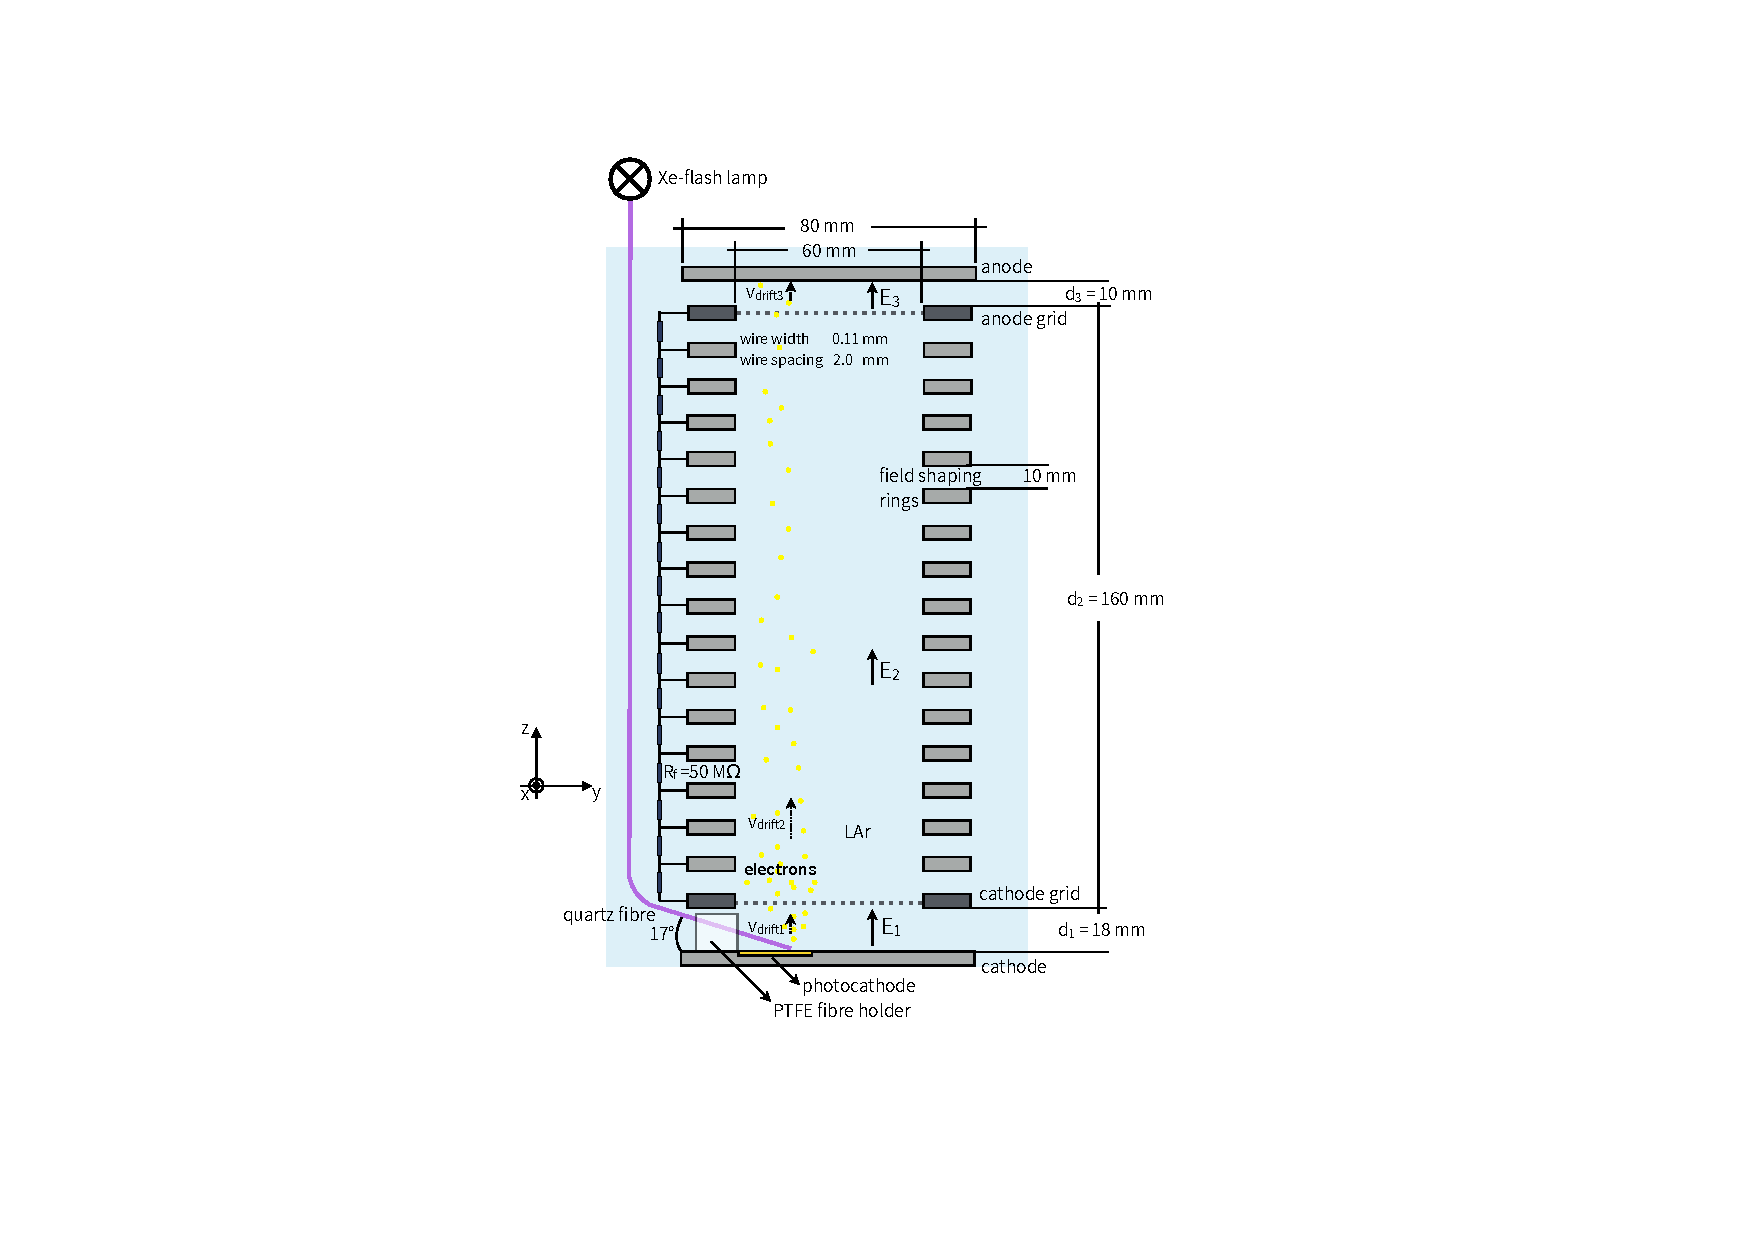
\includegraphics[width=0.95\textwidth, trim={6cm 4.5cm 7cm 2cm}, clip=true]{figures/schematic_purity_monitor.pdf}			
	\caption[]{Schematic drawing of the purity monitor. Measurements are only approximate. For simplicity, only one of the three cathodes is represented.}
	\label{fig:schematic_PM}
	\end{center}	
\end{figure}

In between cathode and anode, two grids---called ``cathode- and anode- grids''---define the drift region. Both are electroformed nickel meshes (MN73 12.63 LPI nickel mesh by Precision Eforming) pinched between two stainless-steel rings. 
In our design, cathode, cathode-grid, anode-grid, and anode can be biased independently. 
We call $E_1$, $E_2$, $E_3$, and $d_1$, $d_2$, $d_3$ the electric fields and distances between cathode and cathode-grid, in between the grids, and between anode-grid and anode, respectively.  
The purpose of the grids is to shield the cathode and anode from the electrons moving in the drift region (i.e. $d_2$), so that the time over which one needs to integrate the signals at the cathode and at the anode is shortened (the drift time is in the order of ms, whereas the integration time of commercially available preamplifiers is in the 50--\SI{150}{\micro s} range). 
Bunemann et al.~\cite{Bunemann1949} found that the inefficiencies of the cathode-grid and anode-grid at shielding ($\sigma_{1}$ and $\sigma_{2}$, respectively) are
\begin{equation}
    \sigma_{1,2} = \frac{\diff E_{1,2}}{\diff E_2} \approx \frac{d}{2\pi d_{1,2}} \log {\left[\frac{s}{2\pi r}\right]}
\end{equation}
where $E_{1,2}$ and $d_{1,2}$ are the electric field and the distance between the collecting plate and the grid respectively, $r$ is the wire radius, and $s$ is the distance in between wires. In an ideal case ($\sigma_{1,2} = 0$), once the electrons have passed the cathode-grid, none of their line of force (which causes $\diff E_2 \neq 0$) still reaches the cathode, i.e. no signal is induced on the cathode (no change in $E_1$ due to a change in $E_2$). Similarly, the anode-grid shields the anode from any lines of force from the drifting electrons---until the electrons cross the grid. At this point, the number of lines of force on the anode from the electrons starts to increase till the electrons reach the anode, when all their lines of force end on the anode. In reality, as $\sigma \neq 0$ one can typically see a little bit of early signal on the anode (i.e. a few field lines penetrate the anode grid as the electrons approach it). The same effect happens on the cathode, but it is harder to see given $d_1>d_2$ by construction (see Fig.~\ref{fig:schematic_PM} for the geometrical characteristics of the purity monitor). It should be noted that the grids efficiency solely depends on the geometry of the purity monitor ($D$) and the geometrical properties of the mesh ($r$ and $s$). In our case $\sigma_1 =2\%$, while $\sigma_2 =3.5\%$. Bunemann et al. also showed that while acting as a shield, the collecting plate and the grid may be biased in such a way that the grid is ``electrically'' transparent to the drifting electrons, i.e. the electric lines of force by-pass the grid (and so do the electrons, as they diffuse along the lines of force). 
The condition for which all the field lines by-pass the cathode- or anode-grid is
\begin{equation}
    \frac{E_\mathrm{i}}{E_{\mathrm{i}-1}} & = \frac{1+\rho}{1-\rho} \approx 2,
    \label{eq:ratio_fields}
\end{equation}
where $\mathrm{i} = 2,3$ and $\rho & = \frac{2\pi r}{s}$. Given for our particular grid choice the ration in eqn~\ref{eq:ratio_fields} is $\approx 2$, we always ran the purity monitor with $E_3\approx 2 E_2 \approx 4 E_1$.

\begin{figure}
	\begin{center}
	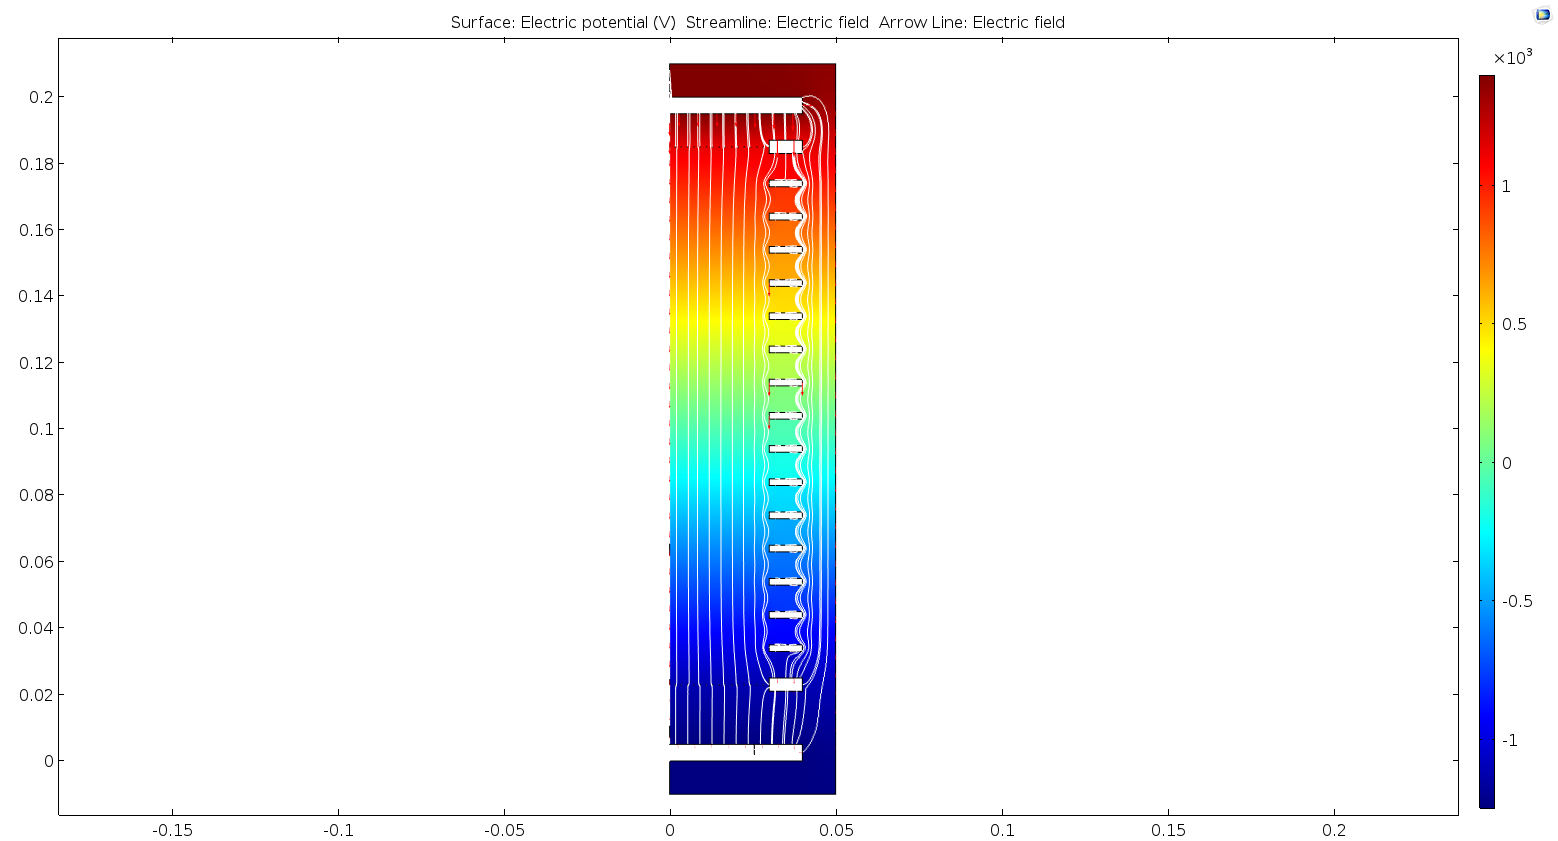
\includegraphics[width=1\textwidth, trim={0 0cm 0cm 0cm}, clip=true]{figures/ComsolForPaper.png}			
	\caption{COMSOL simulation of the purity monitor at an electric field configuration of $\protect \{E_1, E_2, E_3\} = \{70, 140, 280\}\;V/cm$ }
	\label{fig:PnID}
	\end{center}
\end{figure}

In between the two grids, 15 coaxial stainless steel rings interconnected by \SI{50}{\megaohm} resistors act as a field-shaping system to grant electric field uniformity. The COMSOLE simulation shows that the field in the central region is uniform (with field lines perfecty vertical) across the \SI{16}{cm} drift region. Three PEEK rods hold together the electrodes and PTFE spacers separates them. 
The grids are directly connected to a 4-channel power supply from CAEN (model NDT1470). The cathode and the anode are connected to two ORTEC PC142 preamplifiers. The preamplifiers feature a high-voltage input (which is connected to the CAEN power supply) and an output that goes to the oscilloscope (LeCroy 7300A). 

\subsection{The gas system and the chamber}
\begin{sidewaysfigure}
	\begin{center}
	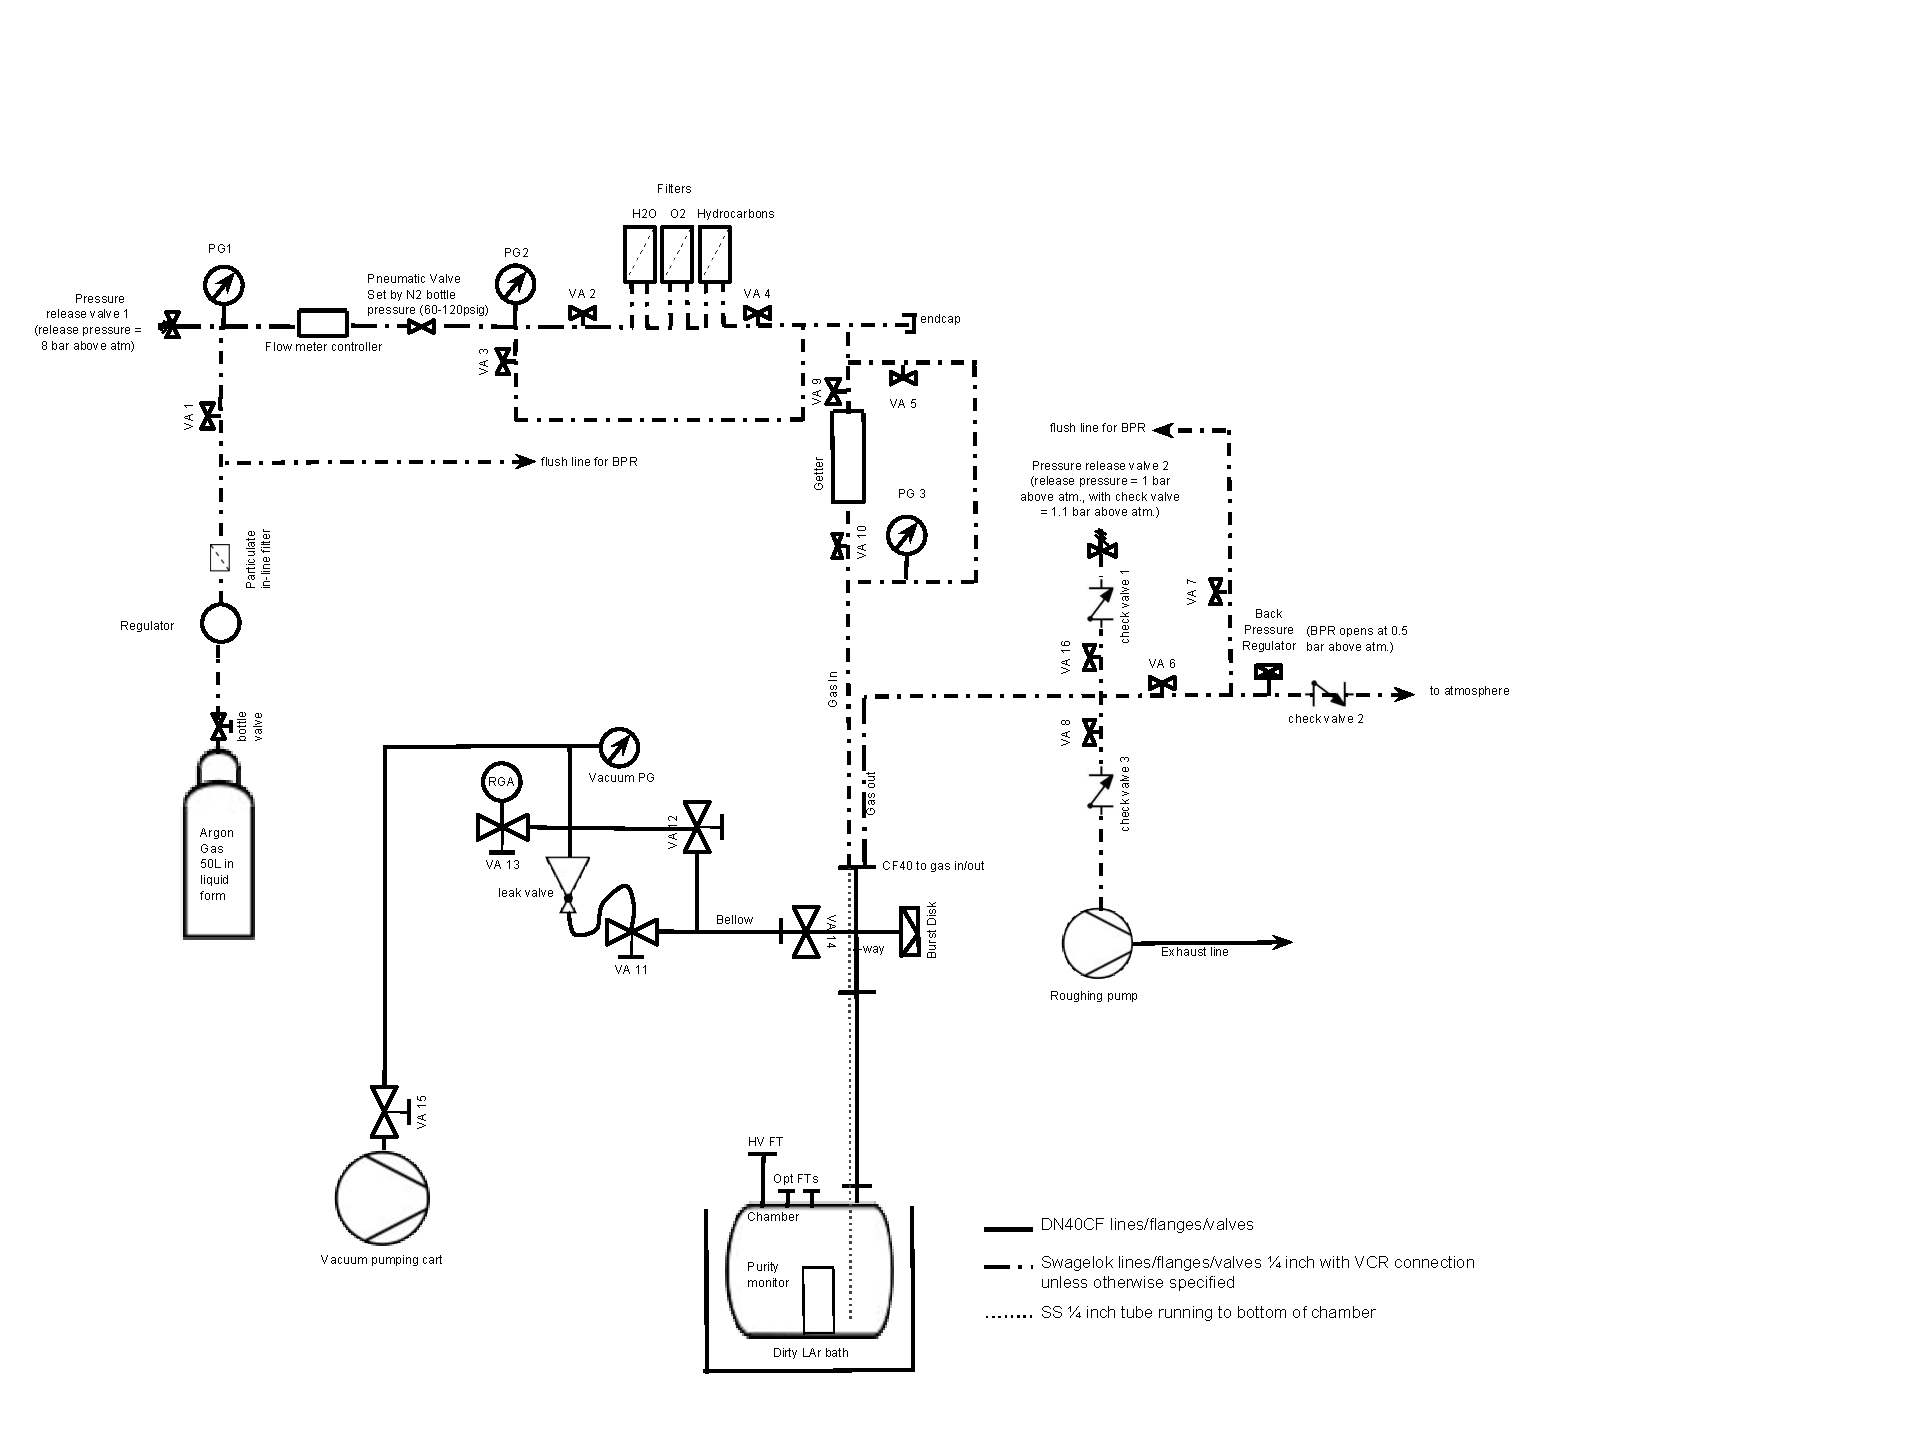
\includegraphics[width=1\textwidth, trim={0 1cm 6cm 2cm}, clip=true]{figures/PnID.pdf}			
	\caption{P\&ID of the LARA test bench gas system to liquify filtered and purified argon gas.}
	\label{fig:PnID}
	\end{center}
\end{sidewaysfigure}

\begin{figure}[tb]
	\begin{center}
	\includegraphics[width=0.9\textwidth]{figures/photo_LARA.jpg}			
	\caption{Photo of the LARA gas system and test chamber. Major components are labelled in the figure.}
	\label{fig:photo_LARA}
	\end{center}
\end{figure}

All tests, in vacuum and liquid argon, have been performed in a dedicated setup at UCL called LARA (Liquid ARgon Apparatus).
Figures~\ref{fig:PnID} shows the the P\&ID (``piping and instrumentation diagram'') of the system, whereas Fig.~\ref{fig:photo_LARA} is a photo of the real setup. Pressurised gaseous argon (GAr) from a commercial N6.0 grade bottle enters the system and is filtered through a SAES MicroTorr getter Model MC50-902F. Table~\ref{tab:airproducts} shows the level of impurities of the GAr according to the supplier (AirProducts). The getter further reduces H\textsubscript{2}O, O\textsubscript{2}, CO, CO\textsubscript{2}, and H\textsubscript{2} up to $<$100\,$ppt$ while acids, bases, and impurities coming from organics and refractory compounds up to $<$10\,ppt. In all our tests the oxygen, moisture, and carbon filters shown in the P\&ID have been by-passed as they restrict the gas flow to 2.5\,SLPM. Instead, only the getter has been used to filter the GAr, resulting in a maximum flow of 10\,SLPM and a liquefaction rate of \SI{23.6}{mm/h} (leading to a total of \SI{9}{hours} for the liquid to reach the top of the anode).
After being filtered the gas argon enters the chamber through a long straight feed-through. Because the chamber (of inner diameter 200\mm\ and height 300\mm) is immersed in an external low-grade LAr bath, the gas inside turns into liquid. 

%%%% TABLE AIR PRODUCTS %%%%
 \begin{table}[tb]
\centering
\caption[]{Level of impurities for N6.0 GAr according to the supplier.}
    
    \smallskip
    \begin{tabular} { ll@{}}
    \toprule
    \multicolumn{1}{l}{Gas} &\multicolumn{1}{l}{Concentration} \\
    \cmidrule(c){1-2}
    O$_2$             & $<10$\,ppb    \\
    H$_2$O            & $<20$\,ppb    \\
    THC$^*$           & $<100$\,ppb   \\
    $\rm CO+CO_2$     & $<50$\,ppb    \\
    N$_2$             & $<0.3$\,ppm   \\
    \multicolumn{1}{l}{\tiny $^*\rm THC = as\; CH_4$} 
    \end{tabular}
    
}\\
    \label{tab:tab:airproducts}
\end{table}
As LARA is not equipped with a recirculation system, it is essential to leak check all connections prior to filling. This is done by using a residual gas analyser, RGA (model Pfeiffer Vacuum Prisma RGA), visible in white above the red cart in the photo. Once the pressure is below $2\times{10^{-4}}$\millibar, a sniffer probe---attached to a helium bottle through a plastic pipe---is scanned over each connection. If any helium sneaks into the vacuum system through a leak, the RGA detects it. All connections---except the ones which are not evacuated and heareby cannot be tested (e.g. the back pressure regulator valve)---showed no leak down to an ion current of $10^{-15}$\,A.  

%%%% LEAK RATE PLOT %%%%
\begin{figure}[tb]
	\begin{center}
	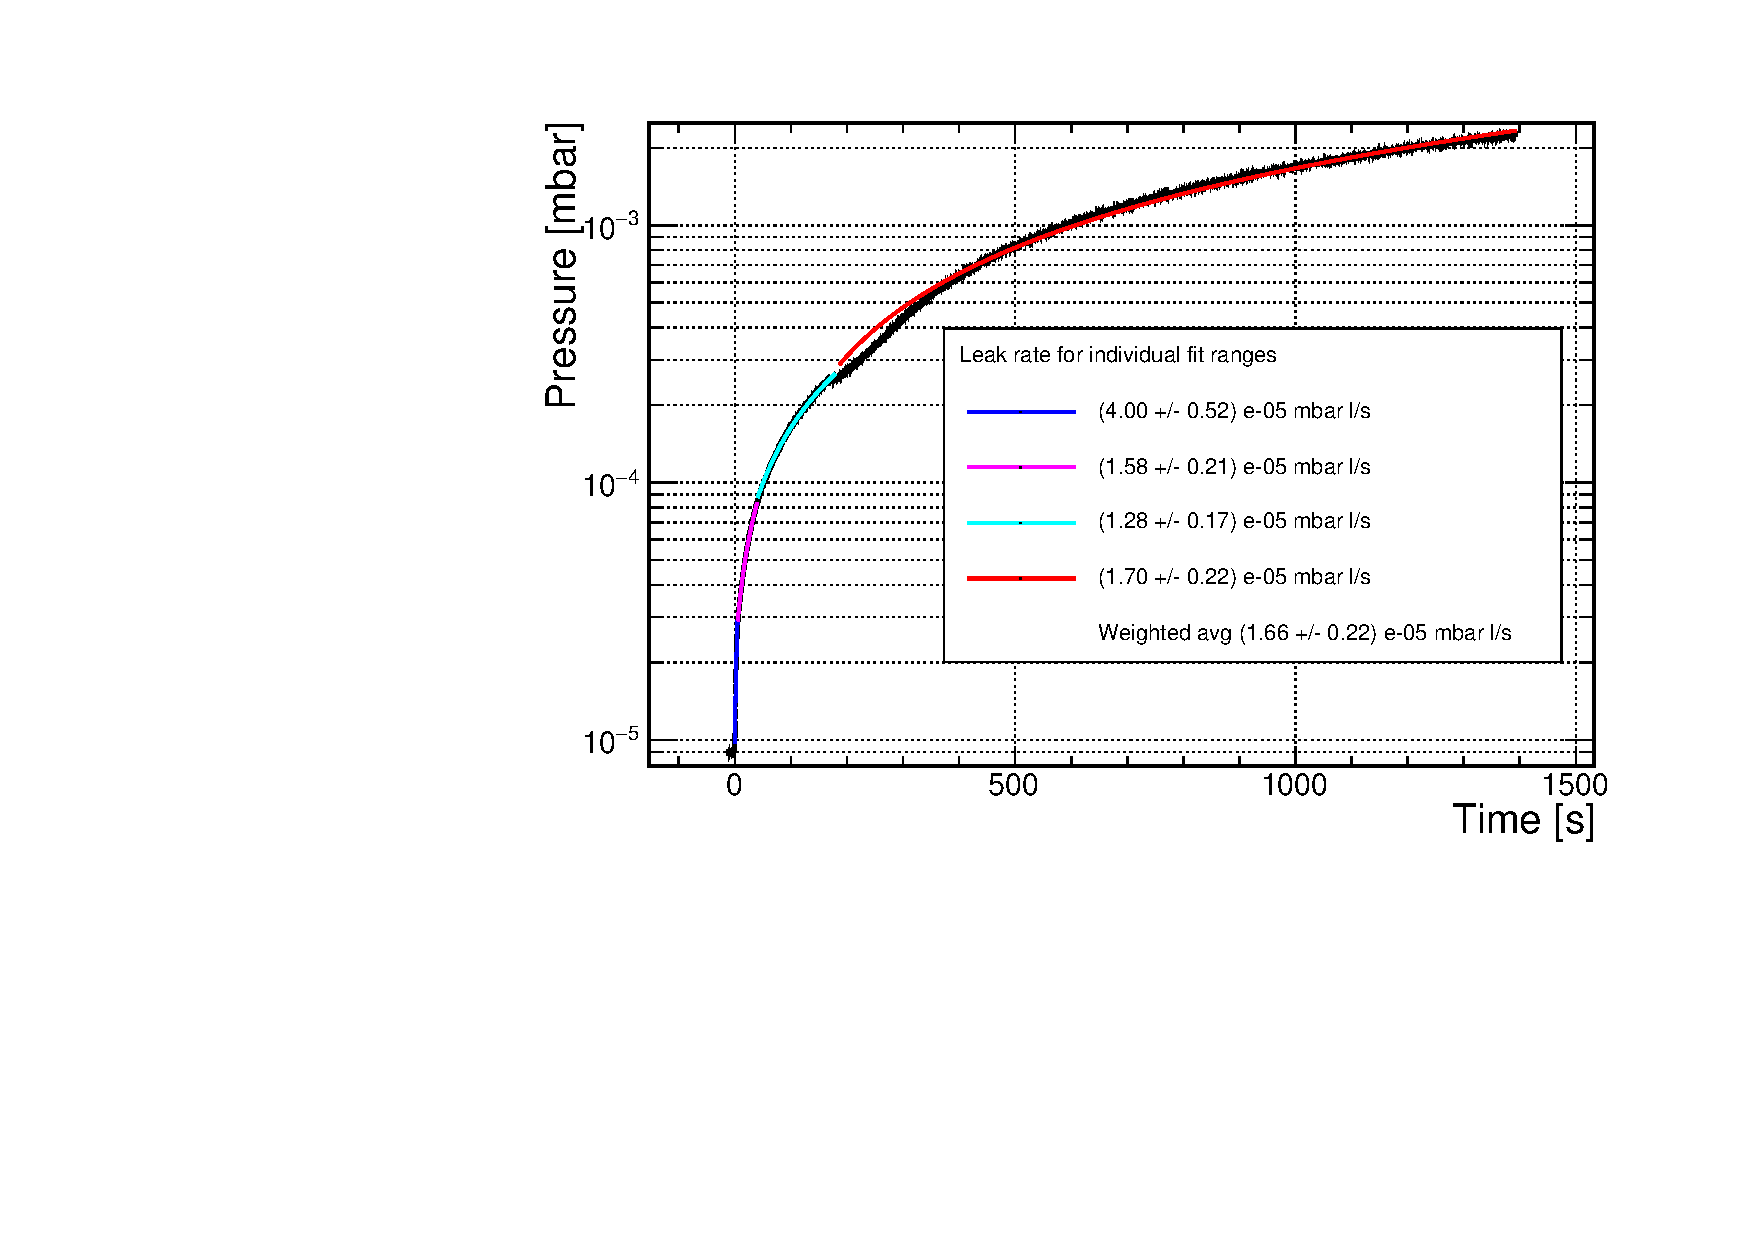
\includegraphics[width=0.9\textwidth]{figures/leak_rate.pdf}}			
	\caption{Rate-of-rise curve to measure the leak rate of our system. A linear fit is applied individually to four ranges (identified by eye) and the weighted mean multiplied by the volume of the setup---chanmber and pipes---is taken as representative of the leak rate of the system. The errors on the fit, pressure measurement and time are all negligible compared to the error on the volume, which alone accounts for 13\%.}
	\label{fig:photo_LARA}
	\end{center}
\end{figure}

A bellow connects the system to the pump cart (model HiCube 80 Eco Pfeiffer Turbo Pump), which can evacuate the chamber down to ${8.9\times10^{-6}}$\,mbar with a leak rate of ${1.6\pm0.1\times10^{-5}}$\millibarL/s when the purity monitor is inside. The error given includes the uncertainty in the calculation of the system volume, fluctuations in the base pressure, the error on the time stamp (negligible) and the error on the fit of the pressure build-up curve.

The liquefaction starts by closing valve 14 (so that the chamber stops being evacuated) and immediately flowing the gas argon into the chamber through the getter. At this point the back pressure regulator (BPR) valve is closed, and so is the pressure release valve---which is only opened when the tests are over and we want the liquid argon to evaporate. Once the pressure inside the chamber (read by the pressure gauge PG3 in the diagram) is around \SI{0.6}{bar} above atmosphere, the BPR is opened and the system is flushed. While purging, the outer bath is filled with low-grade liquid argon. A few minutes later ($\approx$5) the pressure starts dropping: we then know that the gas has started to liquefy and the BPR can then be closed. At that point we monitor that the pressure stays well below \SI{1}{bar} above atmosphere (i.e. when the burst disk would pop) by regulating the flow metre accordingly. Once the liquefaction has stabilised, the pressure is at \SI{0.1}{bar} above atmospheric pressure (provided the cooling power from the outer low-grade argon bath is enough). Originally, the BPR was meant to always stay open when the chamber was pressurised. However, tests have shown that opening the BPR causes some air back flow (despite the check valve), hereby compromising the argon purity.

%**********************************************
\section{Lifetime of electrons in liquid argon}
%**********************************************

%%%%%%%%%%%%%%%%%%%%%%%%%%%%%%%%%%%%%%%%%%%%%%%%
\subsection{Attachment coefficient}
As already mentioned, at each xenon-lamp flash a cloud of electrons is emitted from the cathode and drifted towards the anode. Of the $N_0$ electrons extracted at the cathode, only $N(t_{\rm drift})$ will reach the anode after an average drift time $t_{drift}$, which depends on the average drift velocity $v_{\rm drift}$ at the specific electric field $E$ applied (i.e. $t_{drift} = t_{drfift}(E)$). The electron loss can be parametrised as
\begin{equation}
    N(t_{\rm drift}) = N_0 \eu^{-t_{\rm drift}/\tau}
    \label{eq:electron_loss}
\end{equation}
where $\tau$ is the electron lifetime and $t_{\rm drift} = d/v_{\rm drift}$, with $d$ being the drift distance. Note that equation~\ref{eq:electron_loss} is only approximate, as in reality the presence of a cathode- and anode-grid complicates things slightly.
The electron lifetime is given by
\begin{equation}
    \tau = \frac{1}{\sum_{\rm i} k_{\rm i} n_{\rm i}}
    \label{eq:attachement}
\end{equation}
where the summation runs over the type of electronegative impurities; $k_i$ is the attachment coefficient specific to the impurity $i$ in units of volume per time (usually \si{\liter /(mol.s)} or \si{cm^3/s}); and $n_i$ is the concentration of the specific impurity $i$ in units of inverse volume (usually \si{mol/\liter} or \si{1/cm^3}).  
The electron attachment to an impurity $S$ is described by the following 3-body process: is~\cite{EmissionDetectorsBook}:
\begin{equation}
    \begin{aligned}
    \eu^- + S      & \rightarrow {S^-}^* \\
    {S^-}^* + X & \rightarrow S^- + X
    \end{aligned}
    \label{eq:Block-Broadbury}
\end{equation}
where $X$ is the atom (or molecule) representing most of the medium population (argon in this case) and plays the role of the third body, stabilising the transient negative ion by dissipating the binding energy of the electron. 
The rate of a 3-body attachment process is described by the following equation:
\begin{equation}
    \frac{\diff n_{\eu^-}}{\diff t} = - k^{}_{3} \; n^{}_{\!S} \; n^{}_{X} \; n^{}_{\eu^-}
    \label{eq:att_rate}
\end{equation}
where $n_{\eu^-}$, $n^{}_{\!S^-}$, and $n^{}_{X}$ are the densities of impurities of type $S$, atoms/molecules of the medium, and free electrons respectively. $k^{}_3$ is the 3-body attachment rate of electrons specific to the reaction (i.e. to the type of impurity $S$ and to the atom of the medium $X$).
If $k^{}_3$ does not depend on the density of $S$ nor of that of the medium, then eqn~\ref{eq:Block-Broadbury} can be simplified to a single-stage reaction~\cite{EmissionDetectorsBook}:
\begin{equation}
    e- + S + X \rightarrow S^- + X.
    \label{eq:Block-Broadbury}
\end{equation}
Solving eqn~\ref{eq:att_rate} leads to
\begin{equation}
    \begin{aligned}
    n^{}_{\eu^-} (t) & = n^{}_{0} \exp (-k^{}_3 n^{}_{\!S} n^{}_{X} t) \\
                   & = n^{}_{0} \exp (-t/\tau)                       \\
    \implies \tau  & = \frac{1}{k^{}_3 \: n^{}_{\!S} \: n^{}_{X}},  \\
    \end{aligned}
\end{equation}
where we may absorb $n^{}_{X}$ into the attachment coefficient by defining
\begin{equation}
    k \equiv k^{}_{3} \; n^{}_{X}} 
\end{equation}
so that $k$ has now the dimensions of a volume per time unit. Bakale et al.~\cite{Bakale} reported on the measurement of $k$ for O$_2$ in liquid argon as a function of the electric field and found a slight dependence above \SI{100}{V/cm}.
The reason $k$ does not depend much on the electric field (resulting in the electron lifetime also not being heavily dependent on the field) is because the electron attachment to impurities depends mostly on the electron speed $v =|\Vec{v}|$, which is largely independent of the electric field~\cite{Buckley1989}:
\begin{equation}
    k = \int v\,\sigma(v)\,f(v)\diff v
\end{equation}
where $f(v)$ is the velocity distribution of the electrons---the  Maxwell-Boltzmann distribution, $\sigma (v)$ is the cross-section as a function of the speed for the interaction of the electrons with the impurity $S$.
Assuming oxygen is the main cause of electrons loss in liquid argon, we may write
\begin{equation}
    \tau = \frac{1}{k_{O_2} n_{O_2}}.
\end{equation}
This leads to the following equation for the oxygen equivalent impurity concentration in ppb w/V as a function of the electron lifetime in $\upmu \rm s$:
\begin{equation}
n_{O_2} [\rm ppb\,w/V ] = \frac{\rm ppb\,w/V\, \rm \upmu s}{k\left[\frac{\rm l}{\rm mol\, s}\right] 
31.25 \times 10^{-15} \left[\frac{mol s}{l}\right] \tau[\upmu s]}.   
\end{equation}

%%%%%%%%%%%%%%%%%%%%%%%%%%%%%%%%%%%%%%%%%%%%%%%%
\subsection{Calculation of the electron lifetime}
To calculate the electron lifetime we write $\tau$ as a function of ratio between the charge measured at the cathode and at the anode, and other measurable quantities, namely $t_1$, $t_2$, and $t_3$, i.e. the time to go from cathode to cathode-grid, from cathode-grid to anode-grid, and from anode-grid to anode. 
The cathode and anode currents are calculated as follows:
\begin{align}
    I_{\rm C} & = \frac{Q_0}{d_1}v_{1}\exp\left({-t_{1}/\tau}\right) \\
    I_{\rm A} & = \frac{Q_0}{d_3}v_{3}\exp\left({-t_{3}/\tau}\right) 
\end{align}
where $Q_0$ is the charge born at the cathode. Not to make the notation heavy, we have dropped the subscript $drift$, so that from now on
\begin{equation}
    \begin{aligned}
    v_{drift,i} & \equiv v_i \\ 
    t_{drift,i} & \equiv t_i    \quad \quad \quad i \in [1,3] 
    \end{aligned}
\end{equation}
Integrating $I_C$ and $I_A$ over the appropriate time ranges gives the charge measured by the preamplifiers at the cathode and at the anode:
\begin{align}
    Q_{\rm C} & = \int_0^{t_1} I_C(t) \diff t = \frac{Q_0 \tau}{t_1} \left (1-\eu^{-\frac{t_1}{\tau}}\right) \\
    Q_{\rm A} & = \int_{t_1+t_2}^{t_1+t_2+t_3} I_A(t) \diff t = 
    \frac{Q_0 \tau}{t_3} 
    \eu^{-\left(\frac{t_1+t_2+t_3}{\tau}\right)}
    \eu^{\frac{t_3}{\tau}}-1
\end{align}
Note that for $I_C$ we integrate the current only up to the cathode-grid, as the grid prevents the preamplifier from ``seeing'' what happens behind. Similarly, for $I_A$.
By taking the ratio of the two charges, we obtain
\begin{equation}
    \frac{Q_{\rm A}}{Q_{\rm C}} = \frac{t_1}{t_3} \frac{\eu^{\frac{t_3}{\tau}}-1}{1-\eu^{-\frac{t_1}{\tau}}}
    \frac{\eu^{-\frac{t_3}{2\tau}}}{\eu^{\frac{t_1}{2\tau}}}
    \exp{\left(-\frac{\frac{t_1+t_2}{2}+t_3}{\tau}\right)}
\end{equation}
which can be rewritten as:
\begin{equation}
    \frac{Q_{\rm A}}{Q_{\rm C}} = \frac{t_1}{t_3} 
    \frac{\sinh(t_3/2\tau)}{\sinh(t_1/2\tau)}
    \exp{\left(-\frac{\frac{t_1+t_2}{2}+t_3}{\tau}\right)}.
    \label{eq:sinh}
\end{equation}
Given $t_{1,3} \ll t_2$, the above equation may be approximated to:
\begin{equation}
    \frac{Q_{\rm A}}{Q_{\rm C}} \approx \frac{t_1}{t_3} 
    \frac{t_3/2\tau}{t_1/2\tau}
    \exp{\left(-\frac{\frac{t_1+t_2}{2}+t_3}{\tau}\right)}
\end{equation}
 which solved for $\tau$ gives
\begin{equation}
    \tau \approx \frac{1}{\ln{Q_{\rm A}/Q_{\rm C}}}\left ( t_2 + \frac{t_1+t_3}{2}\right).
    \label{eq:tau_approx}
\end{equation}
Equation~\ref{eq:tau_approx} does not take into account the ``correction factor'' explained in the appendix. 

%**********************************************
\section{Tests in vacuum}
%**********************************************
\begin{figure}[t]
    \centering
    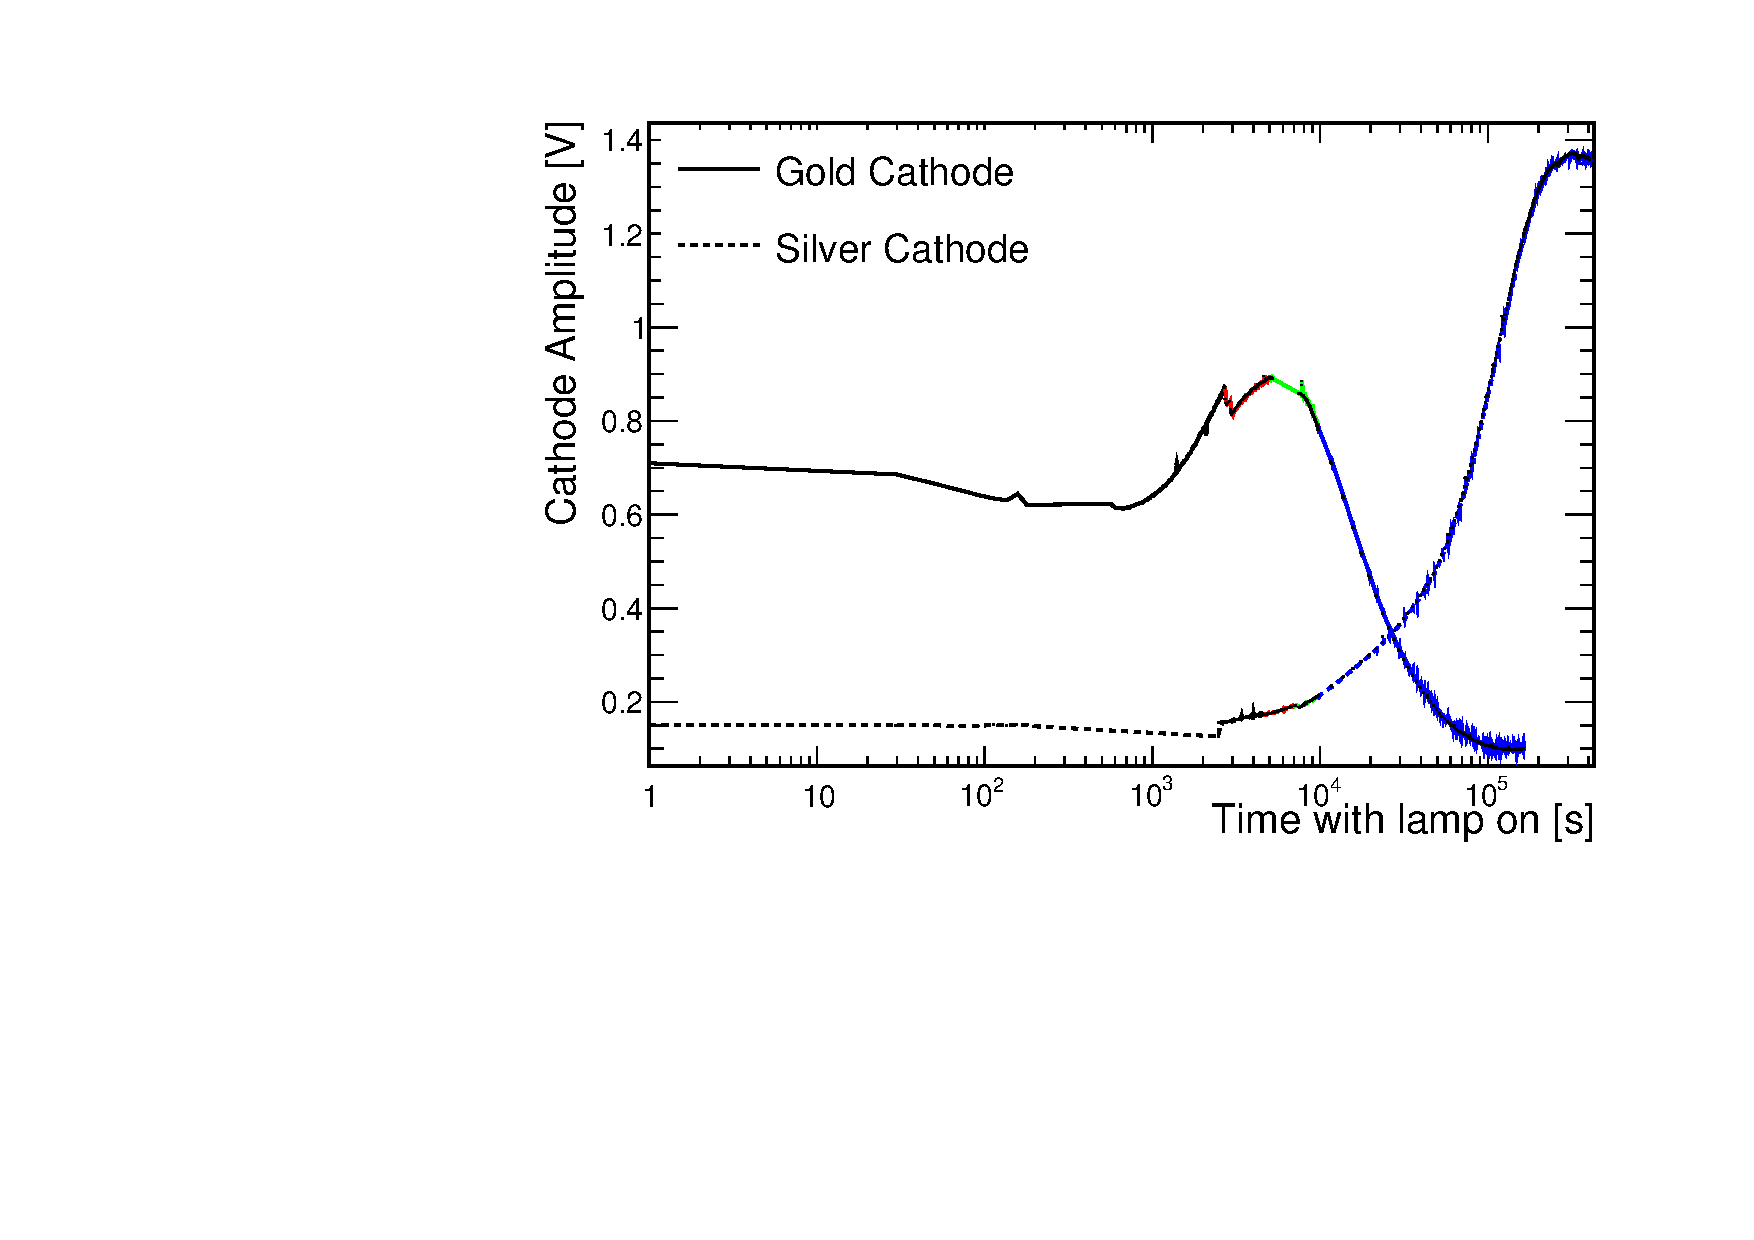
\includegraphics[width=.8\linewidth]{figures/SilverAndGoldVStime.pdf}
    \caption{Vacuum, cathode amplitude (fitted) as a function of time with the lamp on. The discontinuity at 2e3 seconds is because we changed the field from 20.40.80 to -20 20 on just cathode and cathode grid.}
    \label{fig:silver_gold_over_time}
\end{figure}
As the purity monitor is inevitably exposed to air, only materials which do not degrade in atmosphere can be selected for the photocathode. As such, despite their (relatively) high photon-to-electron conversion efficiency (typically $\approx$25--30\%) and low surface barrier, semiconductor compounds commonly used in photomultiplier tubes cannot be used. In contrast to semiconductors, metals are much more resistant to air, but, on the other hand, have much lower quantum efficiency ($\approx$$10^{-5}$--$10^{-4}$\%) and higher surface barriers (typical work functions for metals are \SI{<6}{eV}). In this work we have tested aluminium, titanium, silver, and gold. Aluminium has the lowest work function $\approx$4.1--4.3\,eV~\cite{}), but it is also highly affected by oxidation. The titanium has a slightly higher work function $\approx$4.1--4.3\,eV~\cite{}) and similar oxidation behaviour. The work function of silver exceeds by only a few percent the work function of titanium, but oxidises a lot less. Finally, gold does not react to air, but has a relatively high work function when compared to the other metals.
Being the usual choice for purity monitors in liquid argon (ICARUS, 35 ton...), gold was considered the ``standard'' reference against which all the other materials were compared. 
The first tests have all been conducted in vacuum. As expected Al and Ti showed showed a very small signal compared to the gold sample. Silver instead, albeit smaller, was of the same order of magnitude (NUMBER OF TIMES smaller)  
Hence, we decided to carry out more measurements on silver only. Surprisingly, after \SI{5}{hours} of exposure to the lamp, silver had outgrown gold. Figure~\ref{fig:silver_gold_over_time} shows the behaviour of the metals over time. 

One possible explanation may be that exposure to UV light promotes water vapour outgassing from the photocathode. We tested this hypothesis thtough the chemical analysis of the photocathodes before and after UV light exposure. This was done through energy dispersive X-ray analysis (EDAX) at the London Centre for Nanotechnology. All photocathodes were analysed and then directly exposed to the Xe-flash lamp (no optical fibre, so that the distance to the bulb was only a few mm) for about 30 minutes. 
Figure\ref{fig:EDAX} shows the results for the silver photocathode. This does not explain why, even after one week of exposure to air, silver was still bigger than gold at CERN...
\begin{figure}[t]
    \centering
    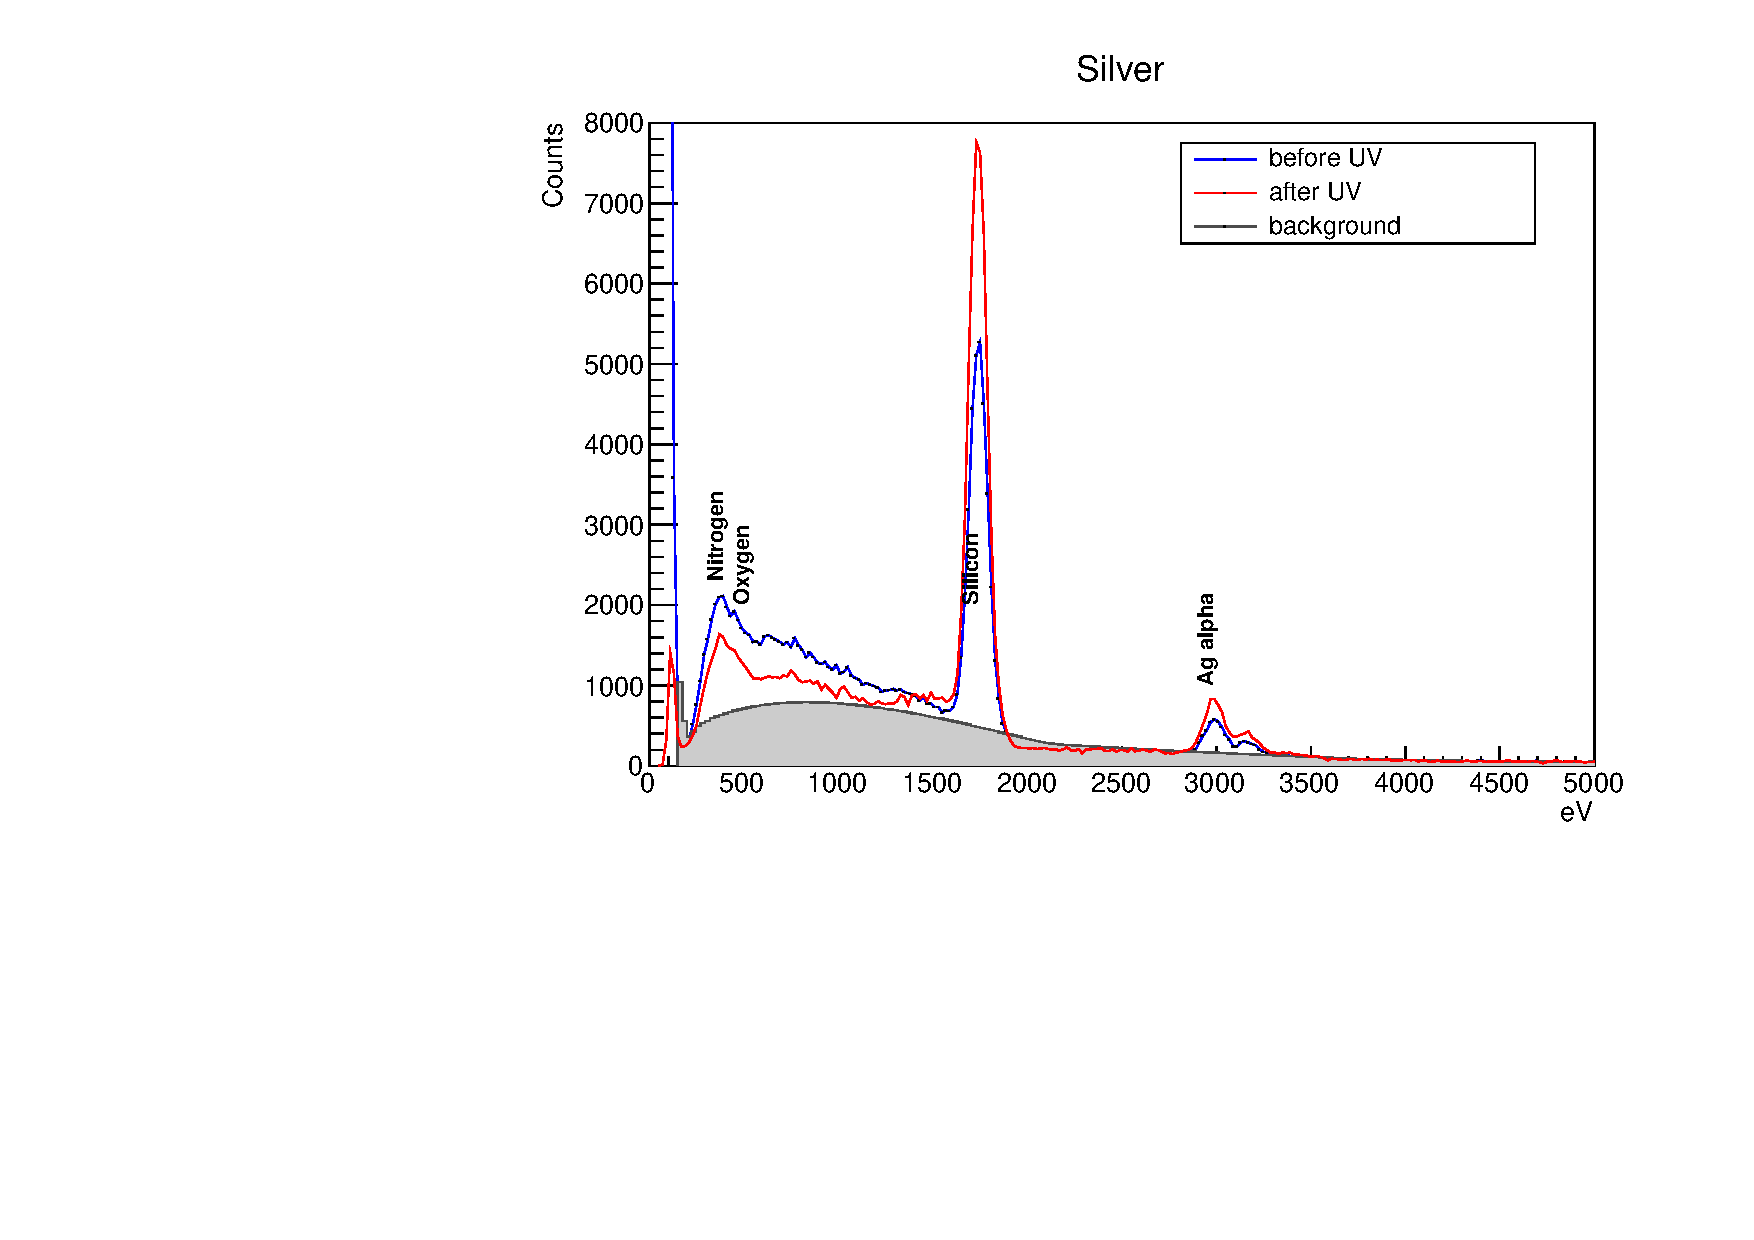
\includegraphics[width=.8\linewidth]{figures/SilverEDAX.pdf}
    \caption{Energy dispersive X-ray analysis of the silver photocathode.}
    \label{fig:EDAX}
\end{figure}

Linda to do:
\begin{itemize}
    \item Ratio of SILVER to GOLD of Amplitude/Integral of average pulse vs time (data of 2018 August 17) 
    \item Ratio of Aluminium to GOLD of Amplitude/Integral of average pulse vs time (old data) 
    \item Ratio of TITANIUM to GOLD of Amplitude/Integral of average pulse vs time (data to be taken)
\end{itemize}

%**********************************************
\section{Tests in liquid argon}
%**********************************************
PLOT that shows RGA measurement of gas argon at room temperature. Is it worth showing?
\begin{figure}[t]
    \centering
    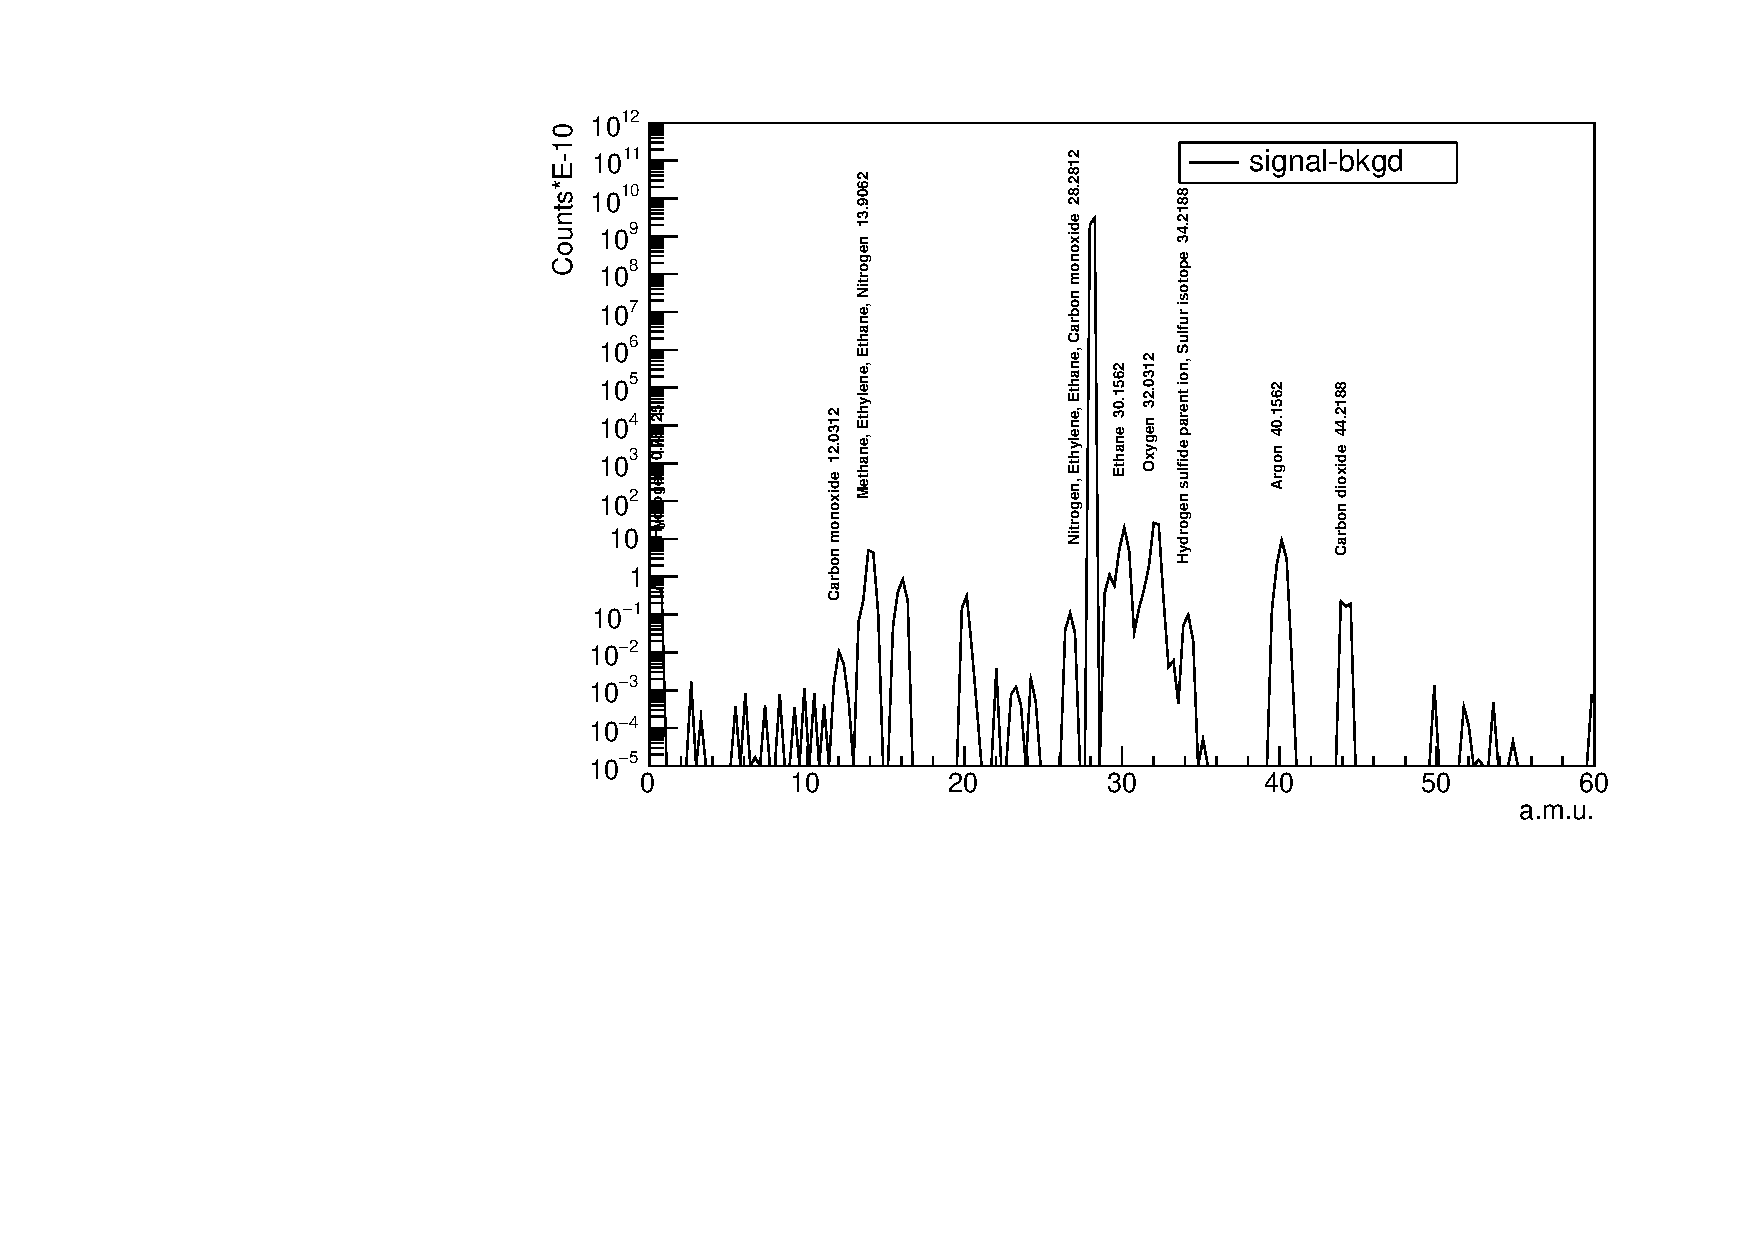
\includegraphics[width=.8\linewidth]{figures/RGAgasscan.pdf}}
    \caption{Energy dispersive X-ray analysis of the silver photocathode.}
    \label{fig:RGAgasscan}
\end{figure}
%**********************************************
\subsection{Measurement of the electron lifetime}
%**********************************************
A sample of 500--1000 waveforms (depending on how noisy is the signal), for both cathode and anode, is saved directly by the oscilloscope and then analysed offline using ROOT. The sample is averaged and smoothing applied. In fact, by making the averaged waveform smoother, it is easier to measure $t_1$, $t_2$, and $t_3$, as well as the minimum and maximum of the cathode and anode amplitudes, respectively (remember that these are the only parameters we need for measuring the electron lifetime). To make our job easier, we also calculate the expected $t_1$, $t_2$, and $t_3$ for the specific electric field applied so that we may know ``ahead'' where to look for the minimum and maximum. Fit?!?

PLOT: data 29.05.2018, show an example of waveform for cathode and anode. Fit anode and cathode min. 

\begin{figure}
    \centering
    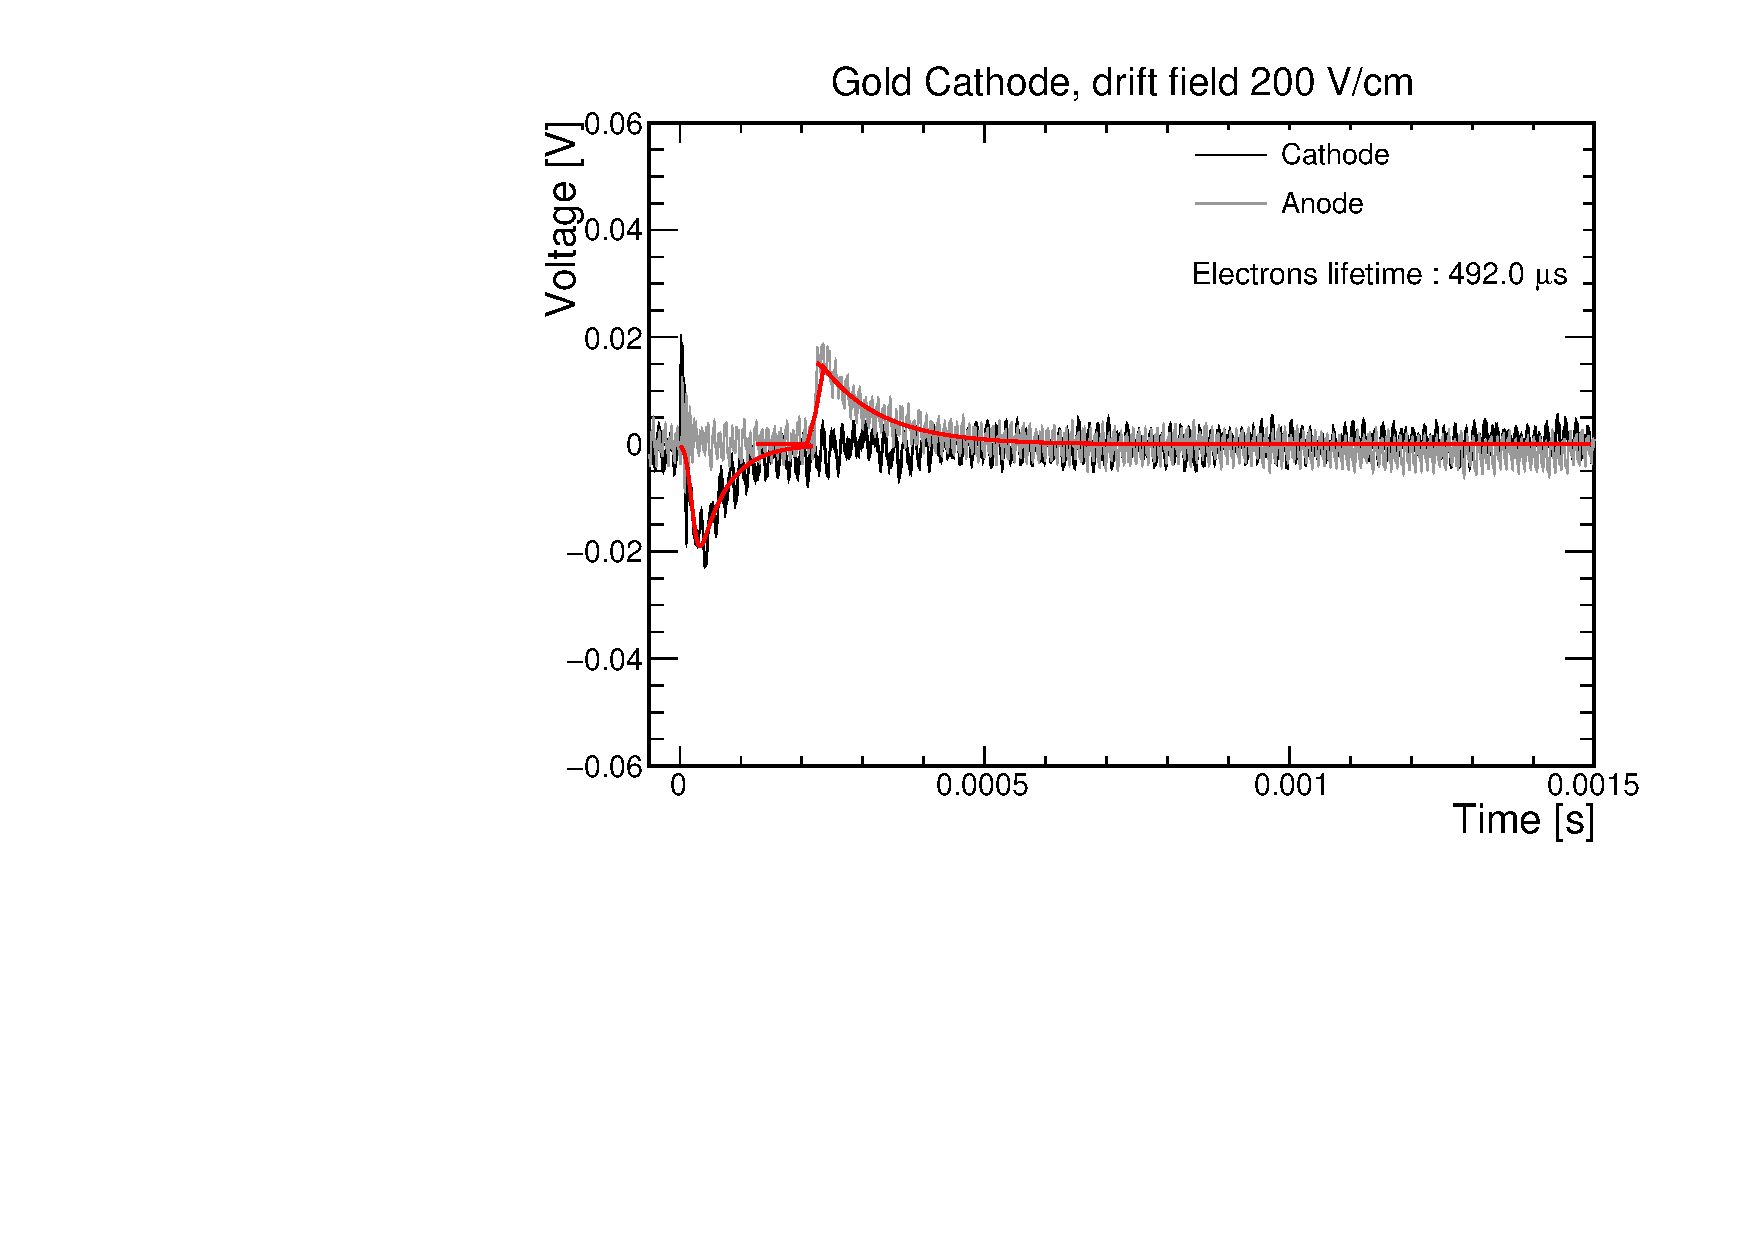
\includegraphics[width=.45\linewidth]{{./figures/SampleWaveformGold_100.200.400Vcm}.pdf} 
    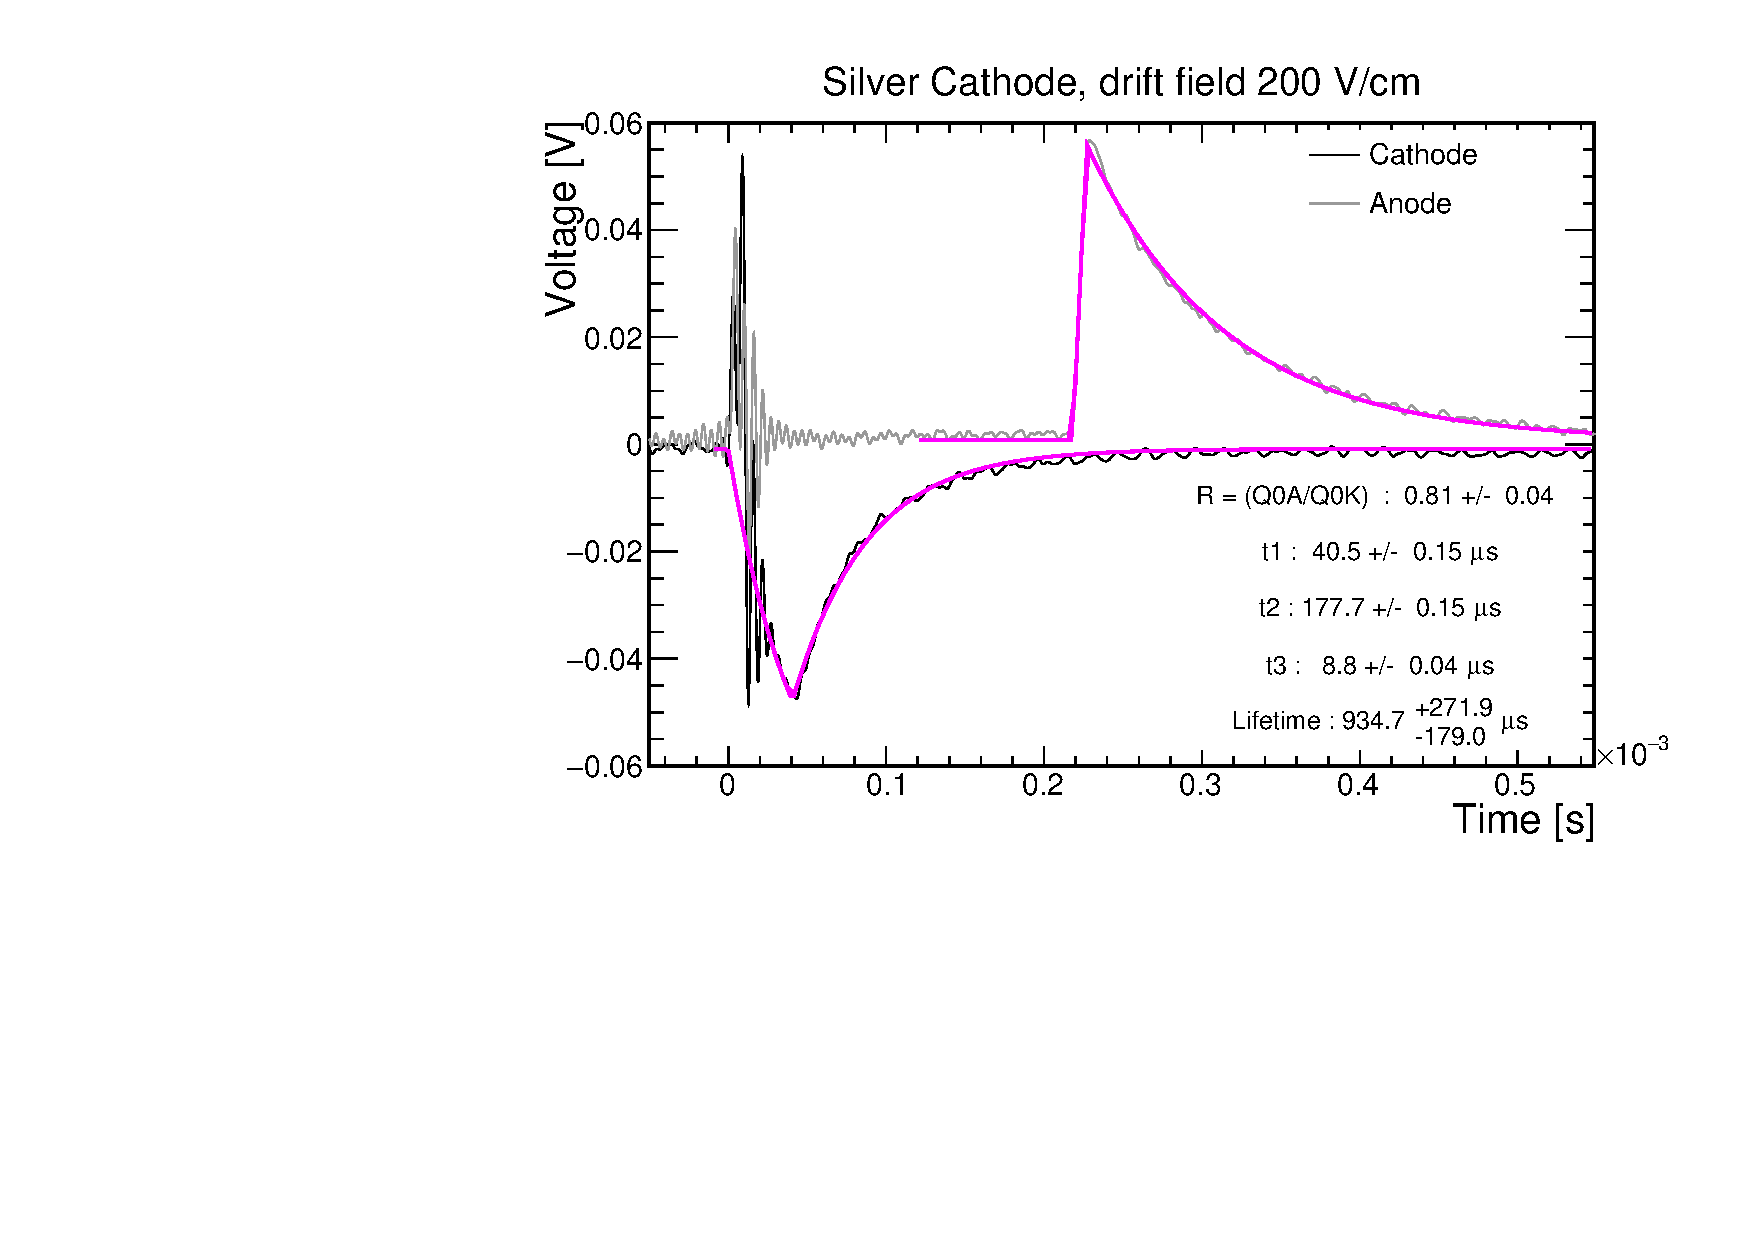
\includegraphics[width=.45\linewidth]{{./figures/SampleWaveformSilver_100.200.400Vcm}.pdf}  \\
        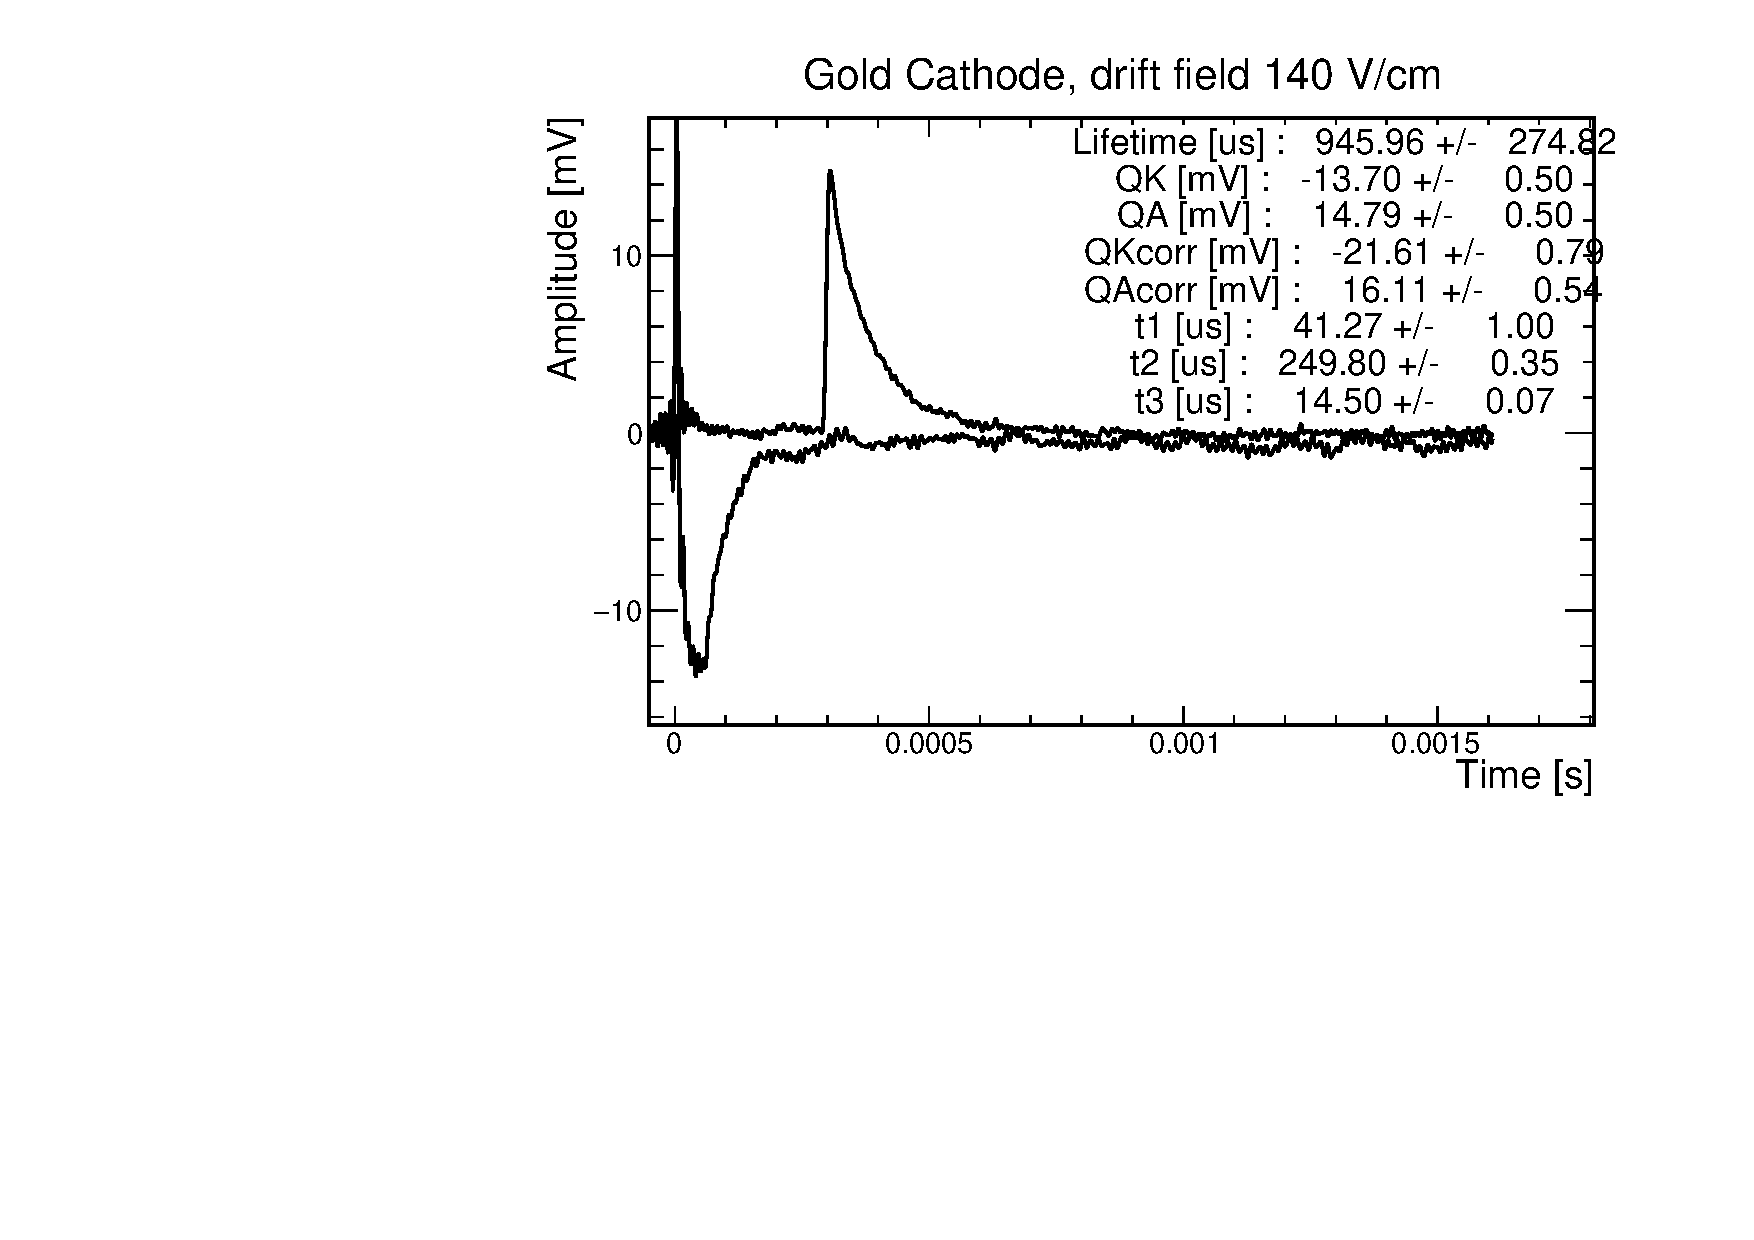
\includegraphics[width=.45\linewidth]{{./figures/SampleWaveformGold_70.140.280Vcm}.pdf} 
    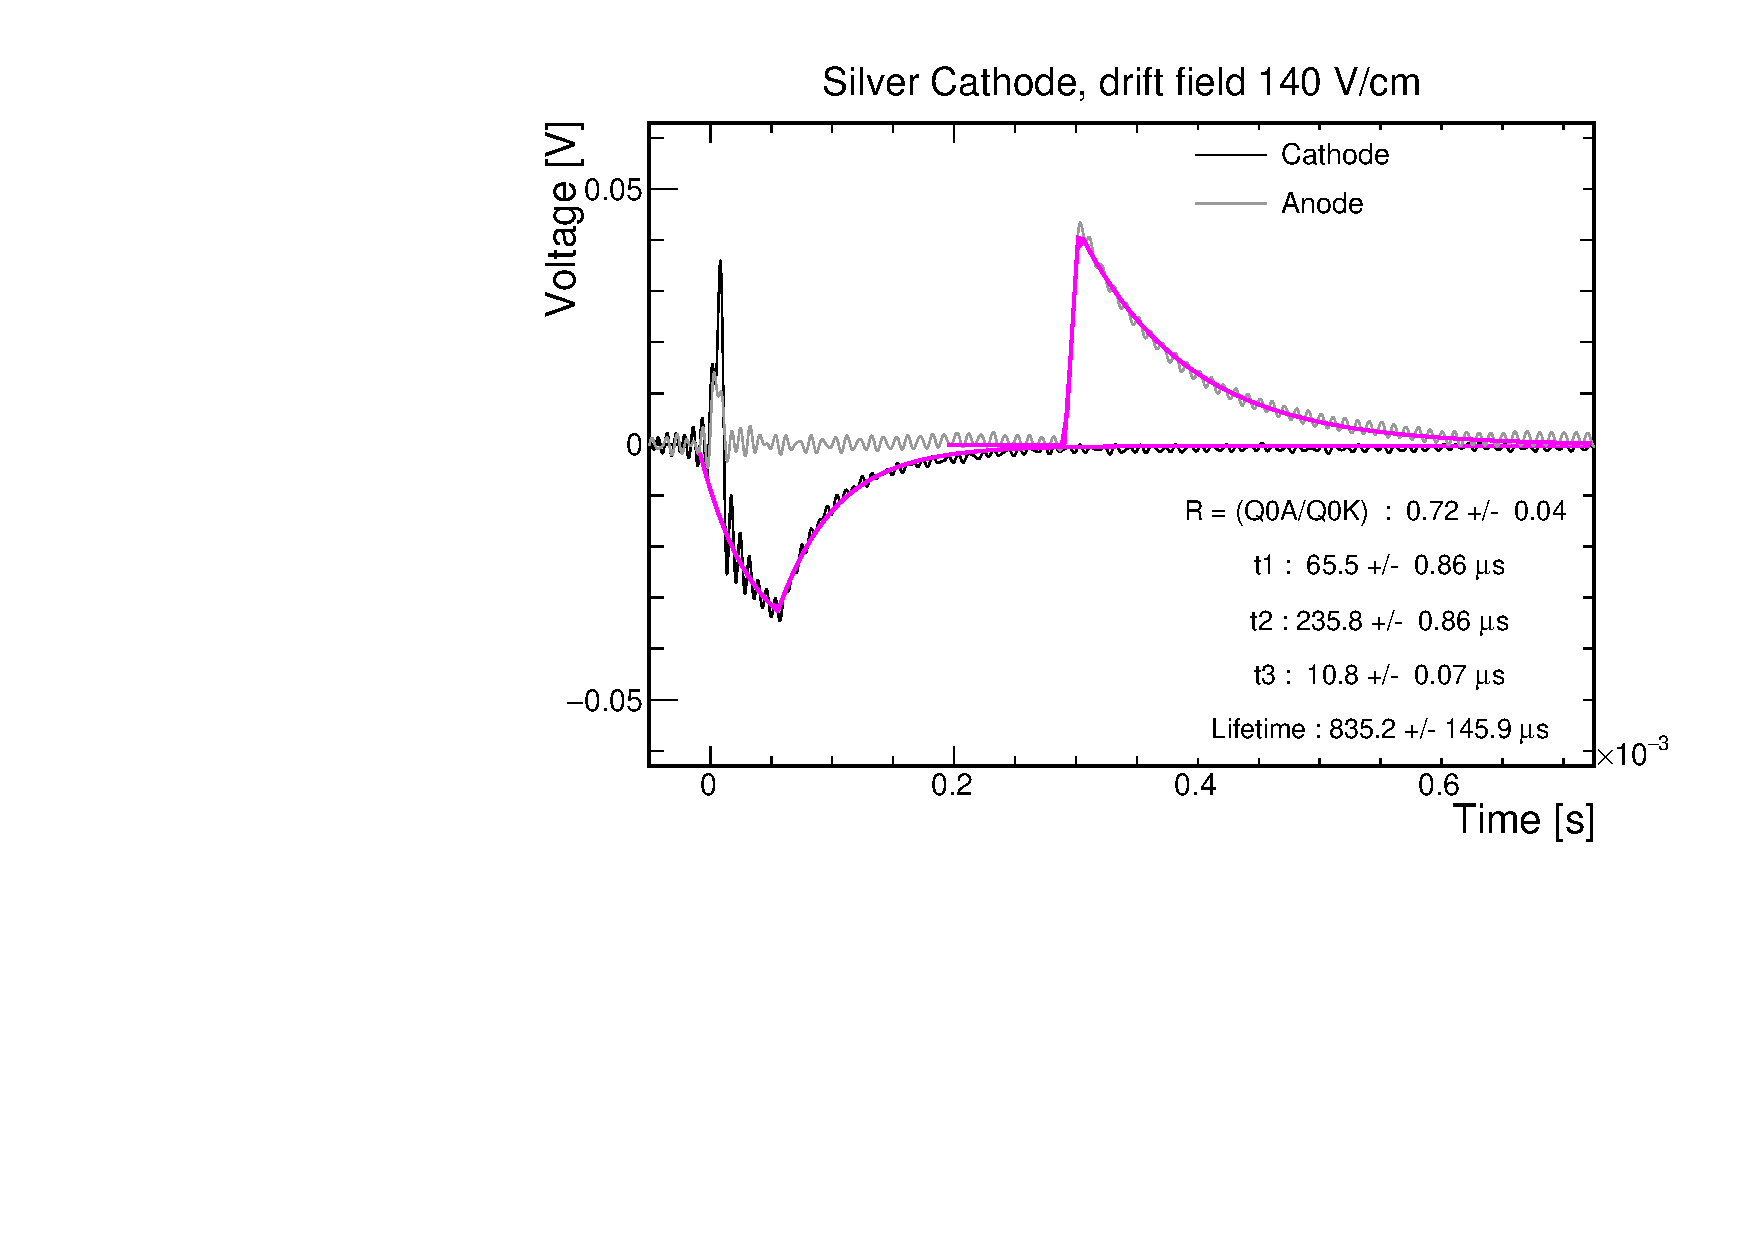
\includegraphics[width=.45\linewidth]{{./figures/SampleWaveformSilver_70.140.280Vcm}.pdf}  \\
        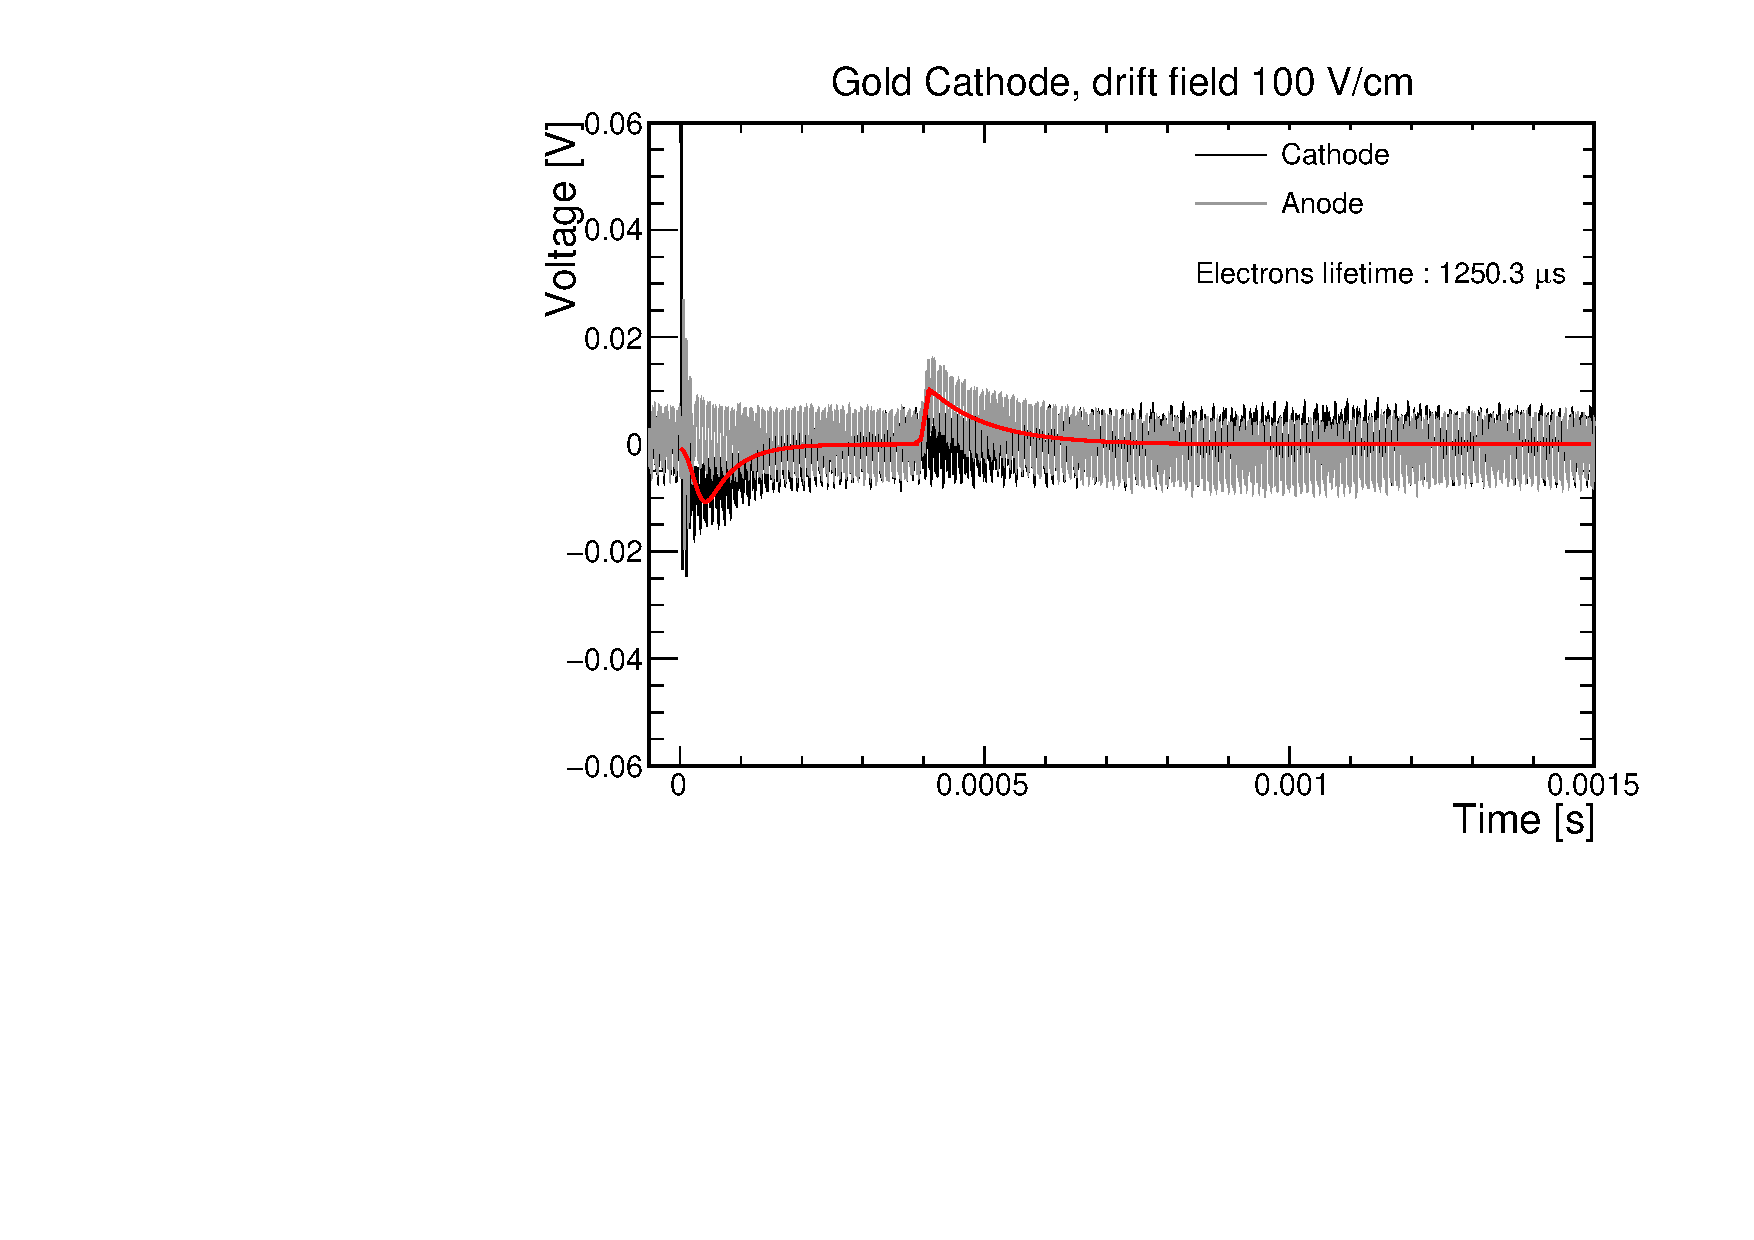
\includegraphics[width=.45\linewidth]{{./figures/SampleWaveformGold_50.100.200Vcm}.pdf}
    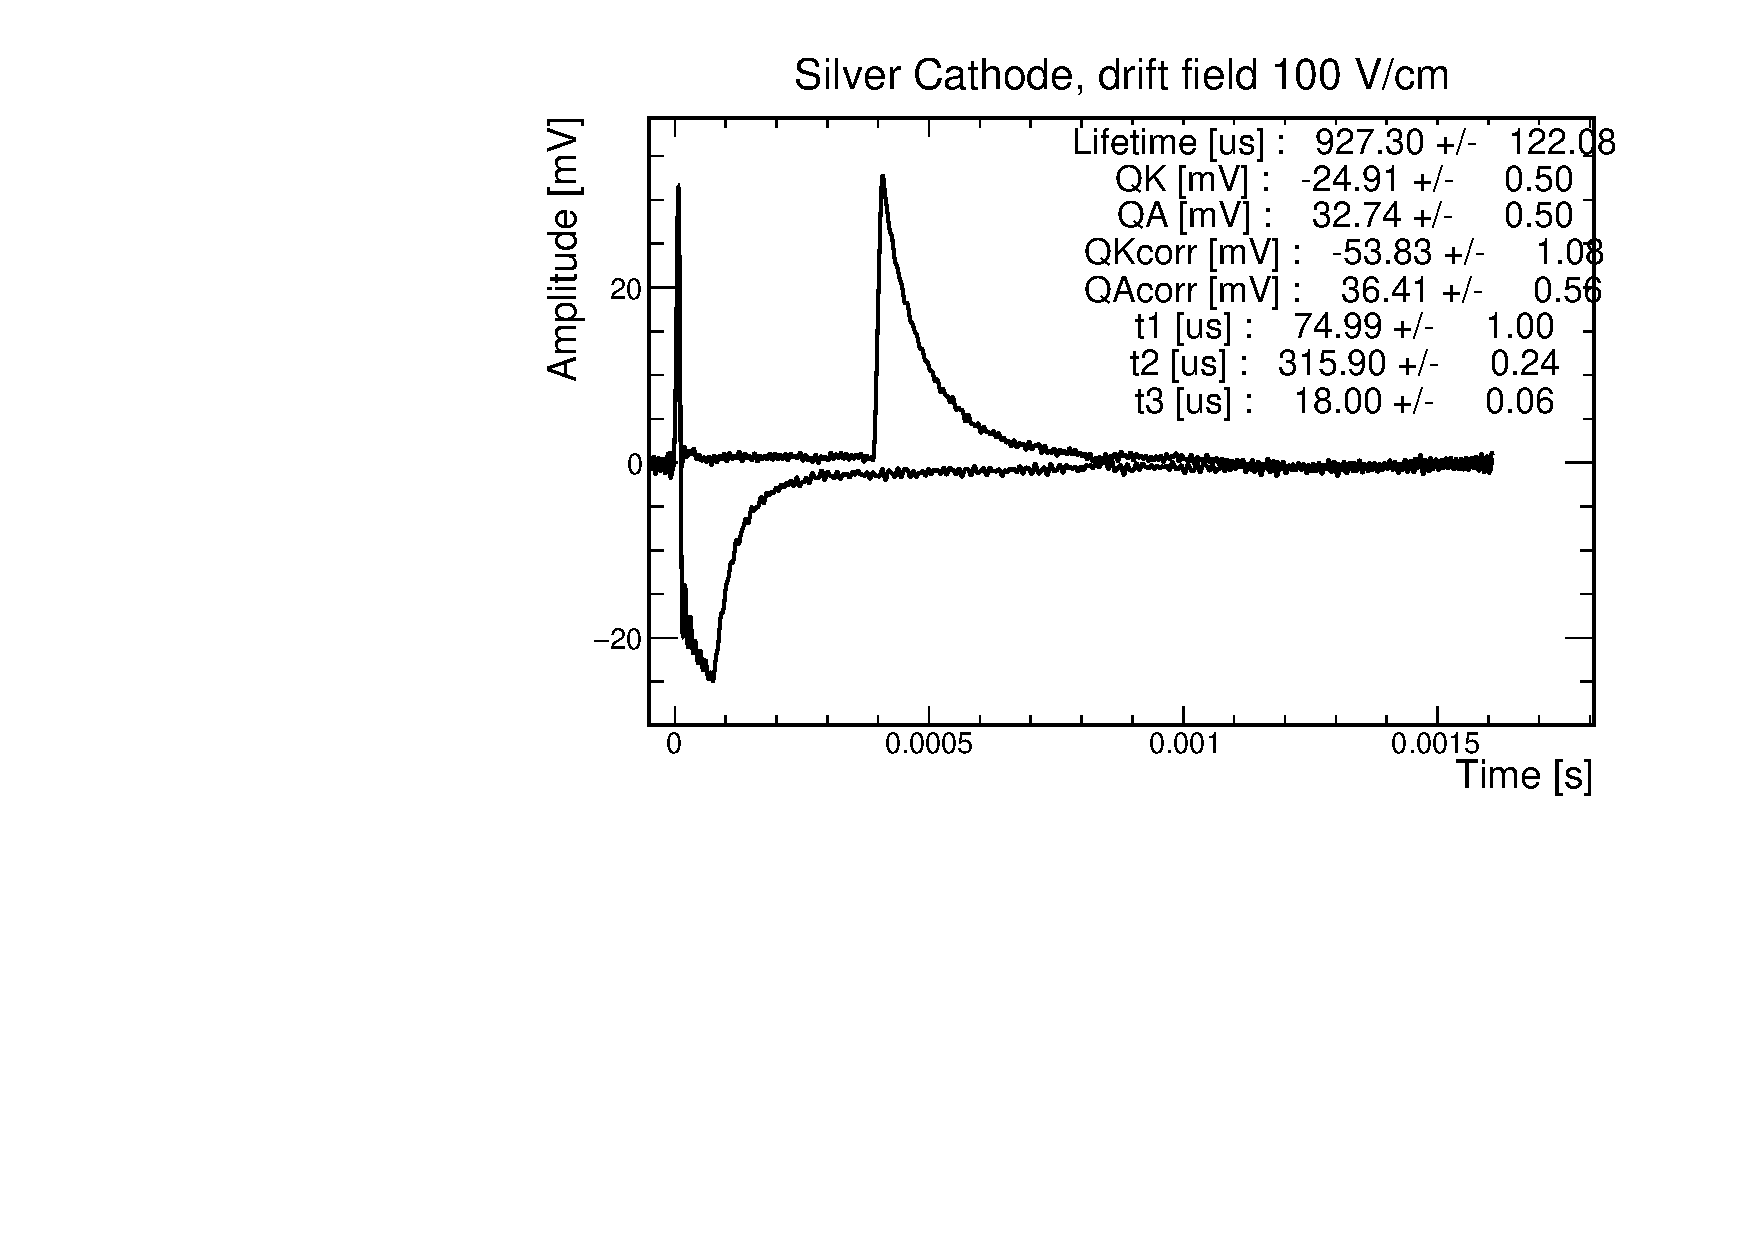
\includegraphics[width=.45\linewidth]{{./figures/SampleWaveformSilver_50.100.200Vcm}.pdf}  \\
        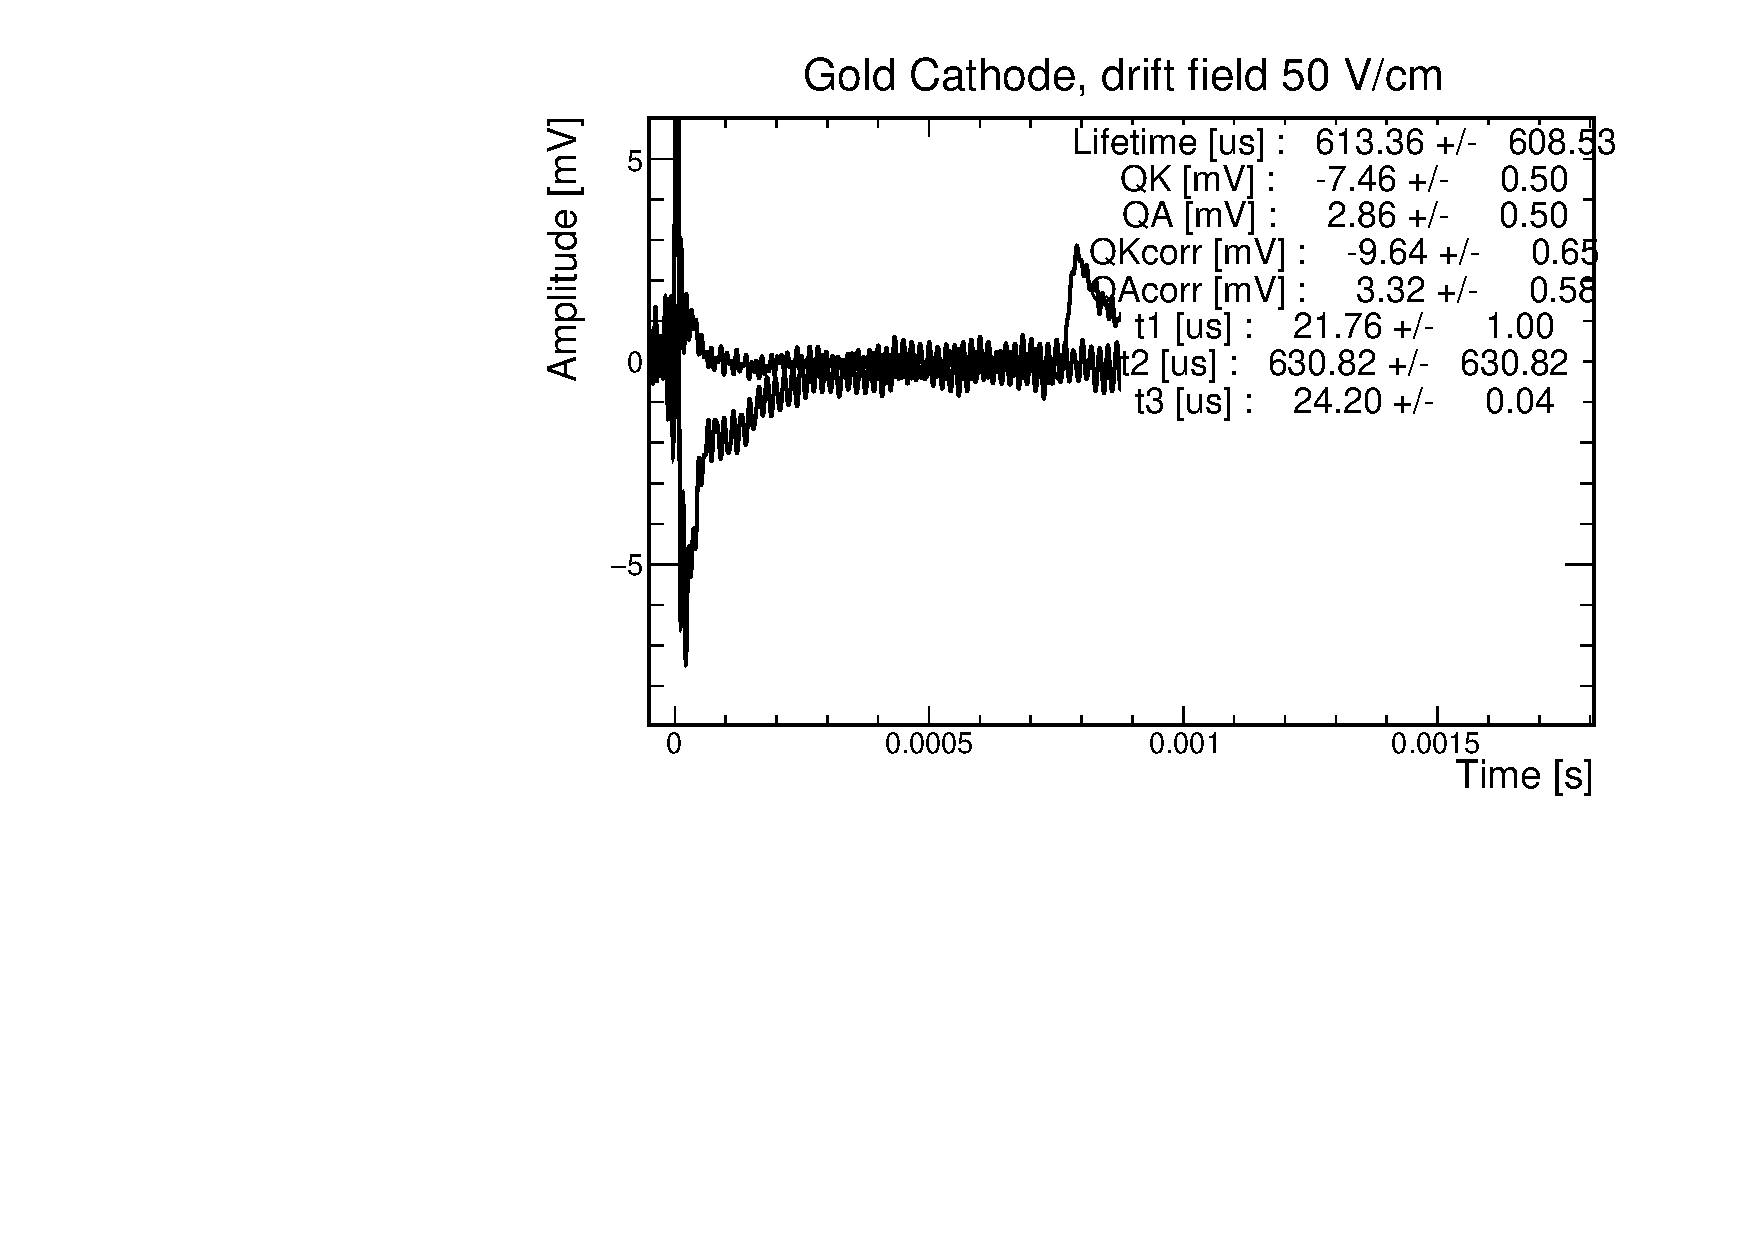
\includegraphics[width=.45\linewidth]{{./figures/SampleWaveformGold_25.50.100Vcm}.pdf} 
    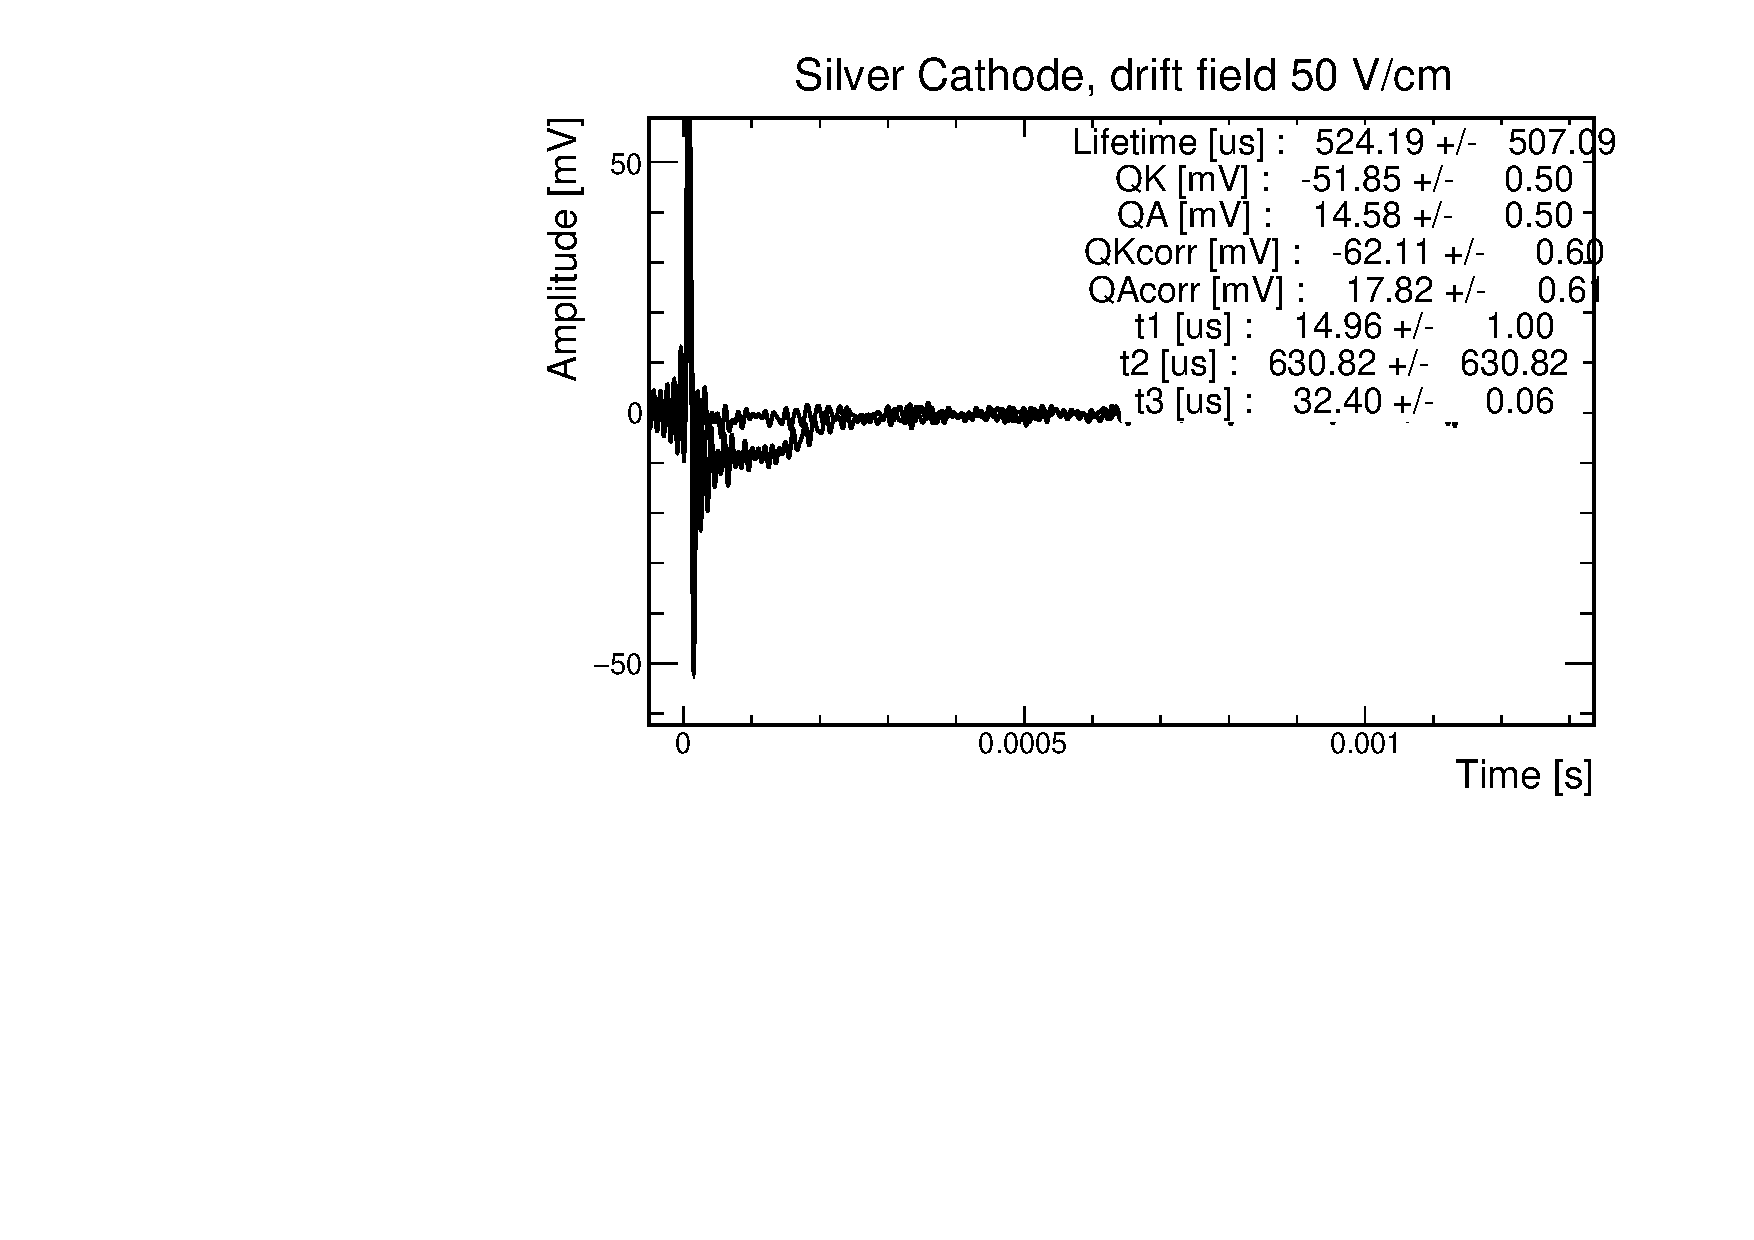
\includegraphics[width=.45\linewidth]{{./figures/SampleWaveformSilver_25.50.100Vcm}.pdf}  \\
    \caption{Liquid Argon example waveforms with gold and silver cathodes. Eventually we will only keep 4 of these plots}
    \label{fig:liquidArgon_GoldVsSilver}
\end{figure}

\subsection{Study of different film depositions in liquid argon}
Silver, silver tarnished with respect to gold. Say about tarnishing etc. 

\subsection{Study at different electric fields}
1 PLOT cathode signal as a function of el field
data of 29.05.2018 and 14.08.2018 and compare (so we see if there is a dependence on the purity)
look at the GK signal, is it the same amplitude as the cathode?
2 PLOT purity as a function of electric field 
3 PLOT Study with long fibre (?): just a waveform and/or purity vs field 

\begin{figure}
    \centering
    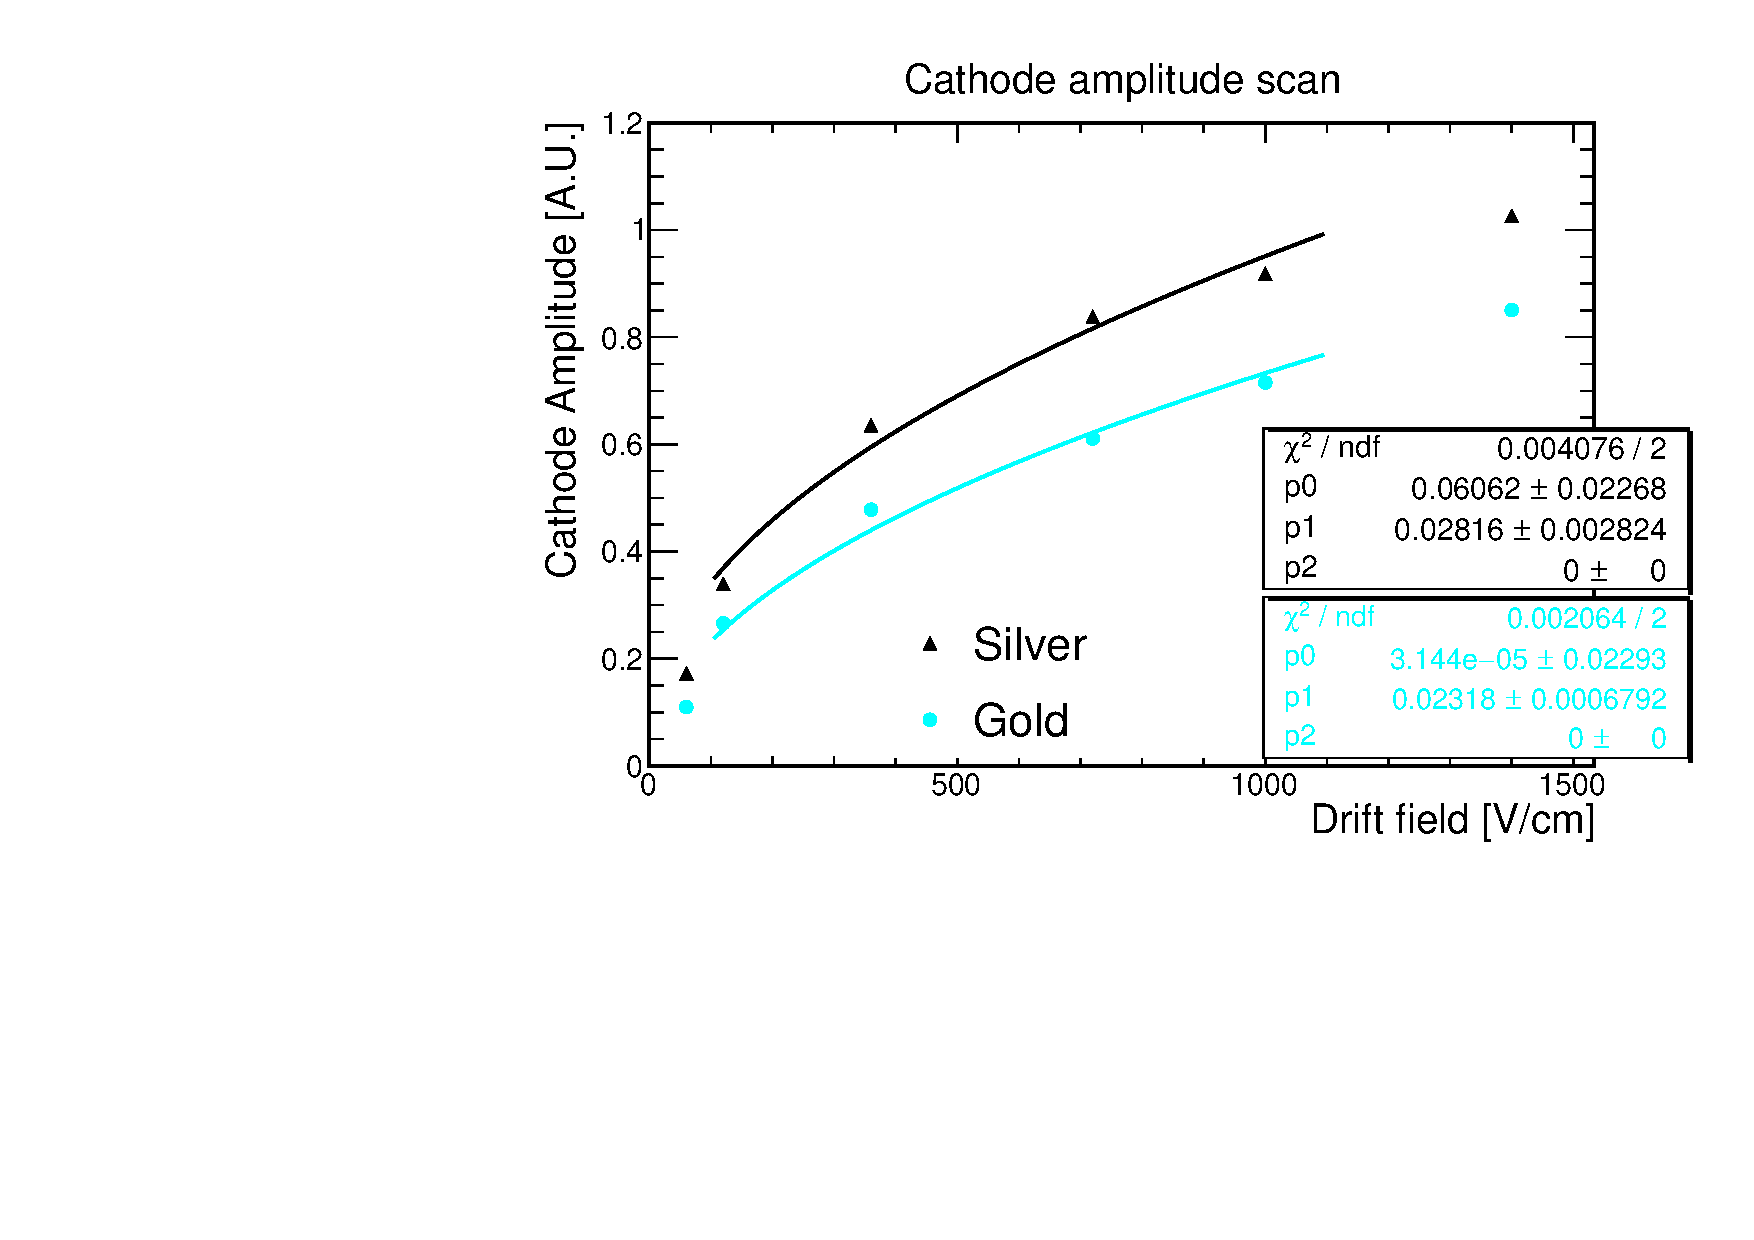
\includegraphics[width=.7\linewidth]{figures/CathodeScan2018Aug14_ShortFibre_SilverGold.pdf}
    \caption{Cathode Scan, data from 2018 August 14. Purity wasn't great but we did take quite a few fields so this worked out.}
    \label{fig:cathodeScan}
\end{figure}

\subsection{Further LAr tests}
It would be good to test the PM (standard size) in LAr again using the modified preamp (longer electronic decay time) and with the photodiode. 

%**********************************************
\section{Conclusions}
%**********************************************

\appendix

%**********************************************
\section{Preamplifier correction factor}
%**********************************************
A charge sensitive preamplifier is an active integrator which takes a current pulse as input and returns a voltage pulse as output. The maximum of the output voltage is proportional to the input charge (i.e. the integrated current). A feedback capacitor $C_f$ between the input and output stores the charge from the detector and amplifies it with gain $1/C_f$ (see later). 

Let us call $g(t)$ the input quantity (current pulse in our case) and $f(t')$ the output quantity (peak of the voltage output in our case). 
In general if the inputs $f_k(t')$ give $g_k(t)$ outputs, then the input $\sum_k c_k f_k (t')$ yields the output $\sum_k c_k g_k (t)$ due to the linearity of the equations describing the circuit. 
Therefore:
\begin{equation}
g(t) = \int \diff t' K(t,t') f(t')
\label{eq:kernel}
\end{equation}
for some function K, called ``kernel''. Electrical circuits usually operate in stationary conditions, hereby we expect that the input $f(t'-t)$ gives the output $g(t-t_0)$, that is to say that if $f$ oscillates with frequency $\omega$, $g$ too will be oscillating with that same frequency. This holds true if the kernel  depends on $t,t'$ through the difference $t-t'$:
\begin{equation}
g(t) = \int \diff t' G(t-t') f(t')
\end{equation}
where $G$ is called ``Green function''. So the output is given by the convolution of the Green function with the input. Incidentally, the Green function is the output observed when the input is $f(t') = \delta(t')$. In this case the convolution gives $g(t) = G(t)$. So when the input current is quick, i.e. the drift time from cathode to cathode-grid is short (this happens when the electric field is high enough), the output voltage is practically the Green function. 

To calculate the charge we need to know the Green function. In RC circuits the Green function is a decreasing exponential (this can be experimentally seen in vacuum for our system):
\begin{equation}
G(t) = G_0 \Theta(t) \eu^{-\frac{t}{RC}}
\end{equation}
where R and C are the resistance and the capacitance of the circuit respectively, and $G_0$ is the gain characteristic of the preamplifier connected to the cathode (note that from a mathematical point of view, $G_0$ is simply a conversion factor, which converts the input charge into a voltage). We can then define $\tau_{\rm el}$ to be the ``electronic decay time'' specific to the system to be:
\begin{equation}
\tau_{\rm el} = RC
\end{equation}
The input function $f(t')$ in eqn~\ref{eq:kernel} is the the current circulating in the preamplifier coming from the detector, which is a step function and for the cathode takes the following form:
\begin{align}
 I_C(t) &=
  \begin{cases}
   \frac{Q_0}{d_1}v_{1}  & 0 \leq t \leq t_{1} \\
   0        			 & t > t_{1}
  \end{cases}
  \label{eq:current_cathode}
\end{align}
Note that we are assuming that the electrons move at constant speed between cathode and grid (i.e. no acceleration) and that after a time $t_1$ they are not seen by the preamplifier anymore due to the shielding property of the grid.
Then, the voltage given by the preamplifier connected to the cathode at any time $t$ is
\begin{equation}
V_{\rm out} (t) = \int \diff t' G(t-t') I_{\rm C}(t')
\label{eq:V_out}
\end{equation}
Doing the integral gives
\begin{equation}
V_{\rm out} (t) = G_0 \frac{Q}{t_1} \tau_{\rm el} \left (1-\eu^{-\frac{t}{\tau_{\rm el}}} \right ) \Theta(t_1-t) \Theta(t)
\end{equation}
Where $I_0 = \frac{Q_0}{d}v_1$. If we fix a value for $t$, then the maximum of this function is reached for $t=t_1$, leading to
\begin{equation}
V_{\rm peak} \equiv V_{\rm out} (t_1) = G_0 \frac{Q_0}{t_1}\tau_{\rm el} \left (1-\eu^{-\frac{t_d}{\tau_{\rm el}}} \right).
\end{equation}
 Therefore $G_0$ has the units of the inverse of a capacitance. This is precisely the feedback capacitance, which, for our preamps, is \SI{0.1}{pF}. 
By rearranging the above equation we get:
\begin{equation}
V_{\rm out} (t_1) = G_0 Q_0 \frac{1-\eu^{-\frac{t_1}{\tau_{\rm el}}}}{\frac{t_1}{\tau_{\rm el}}}
\label{eq:V_final}
\end{equation}
The last factor is the correction that needs to be applied to get the real $V_{peak}$ (need to divide the measure voltage peak by the last factor in the equation above).

Now, $\tau_{\rm el}$ is associated with a physical process (the preamplifier discharging before all the charge has traversed the gird-cathode) which is responsible for an electron depletion. Another process contributes to the electron depletion and this is the electronegative impurities present in the liquid which may trap electrons on their way up from the photocathode to the cathode-grid. The decay time constant associated with this process is what we called earlier $\tau$. To stress the difference between this time constant and $\tau_{\rm el}$, let us rename $\tau \equiv \tau_{\rm life}$.
This means that eqn~\ref{eq:current_cathode} should be rewritten as:
\begin{align}
 I_C(t) &=
  \begin{cases}
   \frac{Q_0}{d_1}v_{1} \eu^{-t/\tau_{\rm life}}  
                            & 0 \leq t \leq t_{1} \\
   0        			    & t > t_{1}
  \end{cases}
  \label{eq:current_cathode}
\end{align}
and integrating again eqn~\ref{eq:V_out} with this new expression for the current, we obtain:
\begin{equation}
V_{\rm out}(t_1) = G_0 Q_0 \frac{
\left(\eu^{-\frac{t_1}{\tau_{\rm el}}}-\eu^{-\frac{t_1}{\tau_{\rm life}}}\right)
}{
\frac{t_{1}}{\left (\frac{1}{\tau_{\rm life}}-\frac{1}{\tau_{\rm el}}\right )^{-1}}
},
\end{equation}
Replacing $t_1$ with $t_3$ and $G_0$ with the specific gain of the preamplifier connected to the anode, gives the maximum amplitude of the signal at the anode. 
We call the factor multiplying the charge and the gain the ``correction factor'' that $V_out$ needs to be divided by to obtain the ``true'' voltage output. Given the gains might be different for the two preamplifiers (as it is in our case), we include $G_0$ in the correction factor too. By including this correction for both cathode and anode, we then obtain the ratio between the ``true'' charge reaching the anode and leaving the cathode. 

\acknowledgments
Lorella and Steve from LCN.

\bibliographystyle{JHEP}
\begingroup
    \setlength{\bibsep}{10pt}
%    \setstretch{1}
    \bibliography{biblio.bib}
\endgroup

\end{document}